%
% FH Technikum Wien
% !TEX encoding = UTF-8 Unicode
%
% Erstellung von Master- und Bachelorarbeiten an der FH Technikum Wien mit Hilfe von LaTeX und der Klasse TWBOOK
%
% Um ein eigenes Dokument zu erstellen, müssen Sie folgendes ergänzen:
% 1) Mit \documentclass[..] einstellen: Master- oder Bachelorarbeit, Studiengang und Sprache
% 2) Mit \newcommand{\FHTWCitationType}.. Zitierstandard festlegen (wird in der Regel vom Studiengang vorgegeben - bitte erfragen)
% 3) Deckblatt, Kurzfassung, etc. ausfüllen
% 4) und die Arbeit schreiben (die verwendeten Literaturquellen in Literatur.bib eintragen)
%
% Getestet mit TeXstudio mit Zeichenkodierung ISO-8859-1 (=ansinew/latin1) und MikTex unter Windows
% Zu beachten ist, dass die Kodierung der Datei mit der Kodierung des paketes inputenc zusammen passt!
% Die Kodierung der Datei twbook.cls MUSS ANSI betragen!
% Bei der Verwendung von UTF8 muss dnicht nur die Kodierung des Dokuments auf UTF8 gestellt sein, sondern auch die des BibTex-Files!
%
% Bugreports und Feedback bitte per E-Mail an latex@technikum-wien.at
%
% Versionen
% *) V0.7: 9.1.2015, RO: Modeline angepasst und verschoben
% *) V0.6: 10.10.2014, RO: Weitere Anpassung an die UK
% *) V0.5: 8.8.2014, WK: Literaturquellen überarbeitet und angepasst
% *) V0.4: 4.8.2014, WK: Initalversion in SVN eingespielt
%
\documentclass[MSE,Master,english]{twbook}%\documentclass[Bachelor,BMR,ngerman]{twbook}
\usepackage[utf8]{inputenc}
\usepackage[T1]{fontenc}

%
% Hier biblatex & Biber konfigurieren; Vergessen Sie nicht, dass Sie biber verwenden müssen um eine Bibliothek zu erzeugen
%
\usepackage[backend=biber, sorting=none, style=numeric]{biblatex}
\addbibresource{Literatur.bib}
\usepackage{float}
\usepackage{pgf-umlsd}
\usepackage{csquotes}
\usepackage{tikz}
\usetikzlibrary{shapes,arrows,positioning}
\usetikzlibrary{positioning}

%
% Bei Bedarf bitte hier die Syntax-Highlightings anpassen
%
\usepackage[final]{listings}
\lstset{captionpos=b, numberbychapter=false,caption=\lstname,frame=single, numbers=left, stepnumber=1, numbersep=2pt, xleftmargin=15pt, framexleftmargin=15pt, numberstyle=\tiny, tabsize=3, columns=fixed, basicstyle={\fontfamily{pcr}\selectfont\footnotesize}, keywordstyle=\bfseries, commentstyle={\color[gray]{0.33}\itshape}, stringstyle=\color[gray]{0.25}, breaklines, breakatwhitespace, breakautoindent}
\lstloadlanguages{[ANSI]C, C++, [gnu]make, gnuplot, Matlab}

%Formatieren des Quellcodeverzeichnisses
\makeatletter
% Setzen der Bezeichnungen für das Quellcodeverzeichnis/Abkürzungsverzeichnis in Abhängigkeit von der eingestellten Sprache
\providecommand\listacroname{}
\@ifclasswith{twbook}{english}
{%
    \renewcommand\lstlistingname{Code}
    \renewcommand\lstlistlistingname{List of Code}
    \renewcommand\listacroname{List of Abbreviations}
}{%
    \renewcommand\lstlistingname{Quellcode}
    \renewcommand\lstlistlistingname{Quellcodeverzeichnis}
    \renewcommand\listacroname{Abkürzungsverzeichnis}
}
% Wenn die Option listof=entryprefix gewählt wurde, Definition des Entyprefixes für das Quellcodeverzeichnis. Definition des Macros listoflolentryname analog zu listoflofentryname und listoflotentryname der KOMA-Klasse
\@ifclasswith{scrbook}{listof=entryprefix}
{%
    \newcommand\listoflolentryname\lstlistingname
}{%
}
\makeatother
\newcommand{\listofcode}{\phantomsection\lstlistoflistings}

% Die nachfolgenden Pakete stellen sonst nicht benötigte Features zur Verfügung
\usepackage{blindtext}

%
% Einträge für Deckblatt, Kurzfassung, etc.
%
\title{Zero Knowledge Proof of owning a Non-Fungible Token (NFT) on the blockchain.}
\author{Rodrigo Manuel Navarro Lajous}
\studentnumber{2120299006}
%\author{Titel Vorname Name, Titel\and{}Titel Vorname Name, Titel}
%\studentnumber{XXXXXXXXXXXXXXX\and{}XXXXXXXXXXXXXXX}
\supervisor{Ing. Gerhard Dinhof, MSc}
%\supervisor[Begutachter]{Titel Vorname Name, Titel}
%\supervisor[Begutachterin]{Titel Vorname Name, Titel}
%\secondsupervisor{Titel Vorname Name, Titel}
%\secondsupervisor[Begutachter]{Titel Vorname Name, Titel}
%\secondsupervisor[Begutachterinnen]{Titel Vorname Name, Titel}
\place{Wien}
\kurzfassung{In den letzten Jahren ist der Schutz der Privatsphäre zu einem immer wichtigeren Thema in der Gesellschaft geworden. Mit dem Aufkommen des Internets, dem großen Boom der Blockchain-Technologie und der Verbreitung persönlicher Daten war die Notwendigkeit, unsere Informationen zu schützen, noch nie so groß. Eine Möglichkeit, die Privatsphäre zu schützen, ist die Verwendung von Zero-Knowledge-Proof. Der Zero-Knowledge-Beweis ist eine mathematische Methode, mit der eine Partei (der Beweisführer) einer anderen Partei (dem Verifizierer) beweisen kann, dass sie eine bestimmte Information kennt, ohne andere Informationen preiszugeben. 

Diese Arbeit zielt darauf ab, das Eigentum an einem Blockchain-basierten nicht-fungiblen Token (eine eindeutige digitale Repräsentation von materiellen oder immateriellen Objekten, in der Regel \ac{NFT}s) zu beweisen, ohne die Identität des Eigentümers preiszugeben. Das Ethereum-Netzwerk, die am weitesten verbreitete Blockchain-Technologie auf dem Markt, wird das Zielsystem sein. Die Arbeit befasst sich mit dem Problem, dass Menschen die Anonymität ihrer digitalen Vermögenswerte wahren müssen. Gleichzeitig können sie mehrere Adressen (digitale Geldbörsen) haben, von denen sie nicht wollen, dass öffentlich bekannt wird, dass sie die Besitzer sind.

Die Schritte zur Lösung dieser Probleme waren theoretische Forschung, Recherche und Auswahl aktueller Rahmenwerke oder Bibliotheken, Entwurf der Lösungsarchitektur, Implementierung und Test. Der erste Teil bestand in der Literaturrecherche und Lektüre. Der zweite Teil bestand darin, das Internet nach dem aktuellen Stand der Technik auf dem Gebiet des Nullwissens zu durchforsten. Außerdem wurde festgestellt, welche Bibliotheken und Frameworks zum Zeitpunkt der Recherche existierten. Nach der Auswahl der Frameworks und Bibliotheken war es im dritten Teil an der Zeit, eine Anwendungsarchitektur zur Lösung des Problems vorzuschlagen. Im vierten Teil wurde die agile Methodik eingesetzt, um mehrere Iterationen des Produkts zu erstellen und es mit den Benutzern zu testen. Schließlich haben wir Usability-Tests und Benchmarks durchgeführt, um die Leistung der Anwendung zu ermitteln.

Eine Schlussfolgerung nach all diesen Schritten ist, dass der aktuelle Stand der Technik von Zero-Knowledge praktische Anwendungsfälle in der realen Welt wie die Generierung des Eigentumsnachweises einer Blockchain-\ac{NFT} ohne Preisgabe der Identität des Eigentümers umsetzen kann. Es gibt jedoch Einschränkungen; angesichts der in dieser Arbeit verwendeten Strategie können wir diese nur statisch und nicht dynamisch nachweisen. Andere Implementierungen können jedoch dynamisch sein, ohne einen Blockchain-Snapshot zu verwenden.
}
\schlagworte{zk-SNARKs, Zero-Knowledge Proofs, Blockchain, Ethereum}
\outline{
In recent years, privacy has become an increasingly important issue in society. With the advent of the Internet, the great boom of blockchain technology and the proliferation of personal data, the need to protect our information has never been greater. One way to achieve privacy is through the use of zero-knowledge proof. Zero-knowledge proof is a mathematical method by which one party (the prover) can prove to another party (the verifier) that they know a particular piece of information without revealing any other information. 

The thesis aims to prove ownership of a blockchain-based non-fungible token (a unique digital representation of tangible or intangible objects, usually \ac{NFT}s) without compromising the owner's identity. The Ethereum network, the most prevalent blockchain technology in the market, will be the targeted system. The thesis addresses the problem of people maintaining the anonymity of their digital assets. At the same time, they may have multiple addresses (digital wallets), of which they do not want to be public knowledge that they are the owners.

The steps to resolve these issues were theoretical research, current frameworks or libraries research and selection, architecture design of the solution, implementation and testing. The first part was researching for a bibliography and reading. The second was scouting the Internet for the current state of the art in the field of zero knowledge. Moreover, seeing which libraries and frameworks exist at the current date of the research. In the third part, once the frameworks and libraries were selected, it was time to propose an application architecture to solve the problem. The fourth part used the Agile methodology to create multiple iterations of the product and test it with users. Finally, we used usability testing and benchmarks to see the application's performance of the product.

A conclusion after all these steps is that the current state of the art of zero-knowledge can implement practical use cases in the real world as generating the proof of ownership of a blockchain \ac{NFT} without compromising the owner's identity. However, it has limitations; given the strategy used in this thesis, we can only prove these in static ways and not dynamically. However, other implementations can be dynamic without using a blockchain snapshot.
}
\keywords{zk-SNARKs, Zero-Knowledge Proofs, Blockchain, Ethereum}
\acknowledgements{
First and foremost, I would like to express my deepest gratitude to my family, especially to my beloved mother and grandparents, for their unwavering support, encouragement, and love throughout my academic journey. Their continuous encouragement and belief in my abilities have been instrumental in my success.

I would also like to extend my sincere appreciation to my alma mater, the Instituto Tecnológico de Buenos Aires (ITBA), for providing me with an outstanding education and a conducive learning environment. The exceptional faculty and staff of ITBA have played an integral role in shaping me into the person I am today.

Furthermore, I would like to express my gratitude to the University of Applied Sciences Technikum Wien for the opportunity to further my education and pursue my passion in computer science. The excellent facilities, faculty, and resources provided by the institution have been invaluable in my personal and professional growth.

I would also like to thank my supervisor, Ing. Gerhard Dinhof, MSc, for his guidance, mentorship, and unwavering support throughout my thesis. His expertise, insights, and constructive feedback have been instrumental in shaping my research.

Last but not least, I would like to thank my colleagues and the team at POAP for their support and for providing me with a challenging and rewarding work experience. Their guidance and mentorship have been crucial in my professional development.
}


\begin{document}

\maketitle

%
% .. und hier beginnt die eigentliche Arbeit. Viel Erfolg beim Verfassen!
%

\chapter{Introduction}
The internet and digital technologies have revolutionised how we live and work. However, it has also created new security, encryption, and anonymity challenges. In this era of global connectivity, data is increasingly vulnerable to theft, leakage, and hacking. All this has led to a heightened need for security and encryption and greater awareness of the importance of anonymity.

Several standard and current problems with security, encryption, and anonymity exist. One of the most significant challenges is the increasing sophistication of cyber-attacks. Hackers are constantly finding new ways to penetrate systems and steal data, making it difficult for businesses and individuals to keep their data safe.

Another problem is the weak security of many internet-connected devices, including everything from laptops and smartphones to home routers and security cameras. Many of these devices are easy to hack into, giving cyber-criminals access to personal and sensitive data. Additionally, outdated security methods, such as password-based authentication and lack of data encryption, continue to be prevalent in many organisations, leaving them vulnerable to attack.

This thesis addresses privacy issues surrounding \ac{NFT} proof of ownership in Ethereum.

\section{Motivation}
Proving ownership of an \ac{NFT} enables various use cases regarding token-gated benefits, such as access to exclusive content, discounts, and participation in events such as conferences, meetup, concerts and so on. However, current methods for proving ownership may inadvertently expose personal information and transaction history, which raises privacy concerns for users. Implementing a more privacy-preserving approach, such as Zero Knowledge Proofs, could enhance the attractiveness and security of \ac{NFT}-based platforms while maintaining the integrity of the blockchain and providing users with increased control over their personal information.

\subsection{The problem}
When a person makes a transaction on the blockchain, that information remains permanently, creating an immutable record. By proving their ownership of an asset, individuals may inadvertently expose sensitive information that can reveal their entire transaction history on the blockchain. This lack of privacy contrasts with other blockchains, such as Bitcoin, which allows users to generate specific addresses for each transaction, thus enhancing their anonymity. With the increasing popularity and adoption of \ac{NFT}s in various industries, the need for privacy-preserving methods of proving ownership has become critical. The challenge lies in developing an approach that maintains the benefits of transparency and decentralisation while protecting users' personal information and ensuring their anonymity.

\section{Main Goals}
This research aims to develop a platform that enables users to access token-gated benefits through Zero Knowledge Proofs, ensuring privacy and anonymity in proving \ac{NFT} ownership. The following objectives will be pursued:

\begin{enumerate}
\item \textbf{Investigate} the current state-of-the-art Zero Knowledge Proofs and their applications in blockchain technology.
\item \textbf{Identify} the challenges and limitations of using Zero-Knowledge Proofs for \ac{NFT} ownership verification.
\item \textbf{Propose} a novel architecture for integrating Zero Knowledge Proofs into \ac{NFT} platforms and ecosystems.
\item \textbf{Develop} a minimum viable product (MVP) that generates proof of \ac{NFT} ownership without revealing personal information. The MVP will involve a user sending a proof request to a verifier (e.g., a bouncer), who will then compare the user's response with the expected proof, ensuring a match without disclosing sensitive information.
\end{enumerate}

By achieving these goals, this research aims to contribute to the ongoing development of privacy-preserving methods in blockchain technology, specifically in \ac{NFT} ownership verification.

\section{Research Questions}
Before formulating the hypothesis, the following research questions were explored:

\begin{enumerate}
\item Is there a way to prove ownership without personal information?
\item What is Zero Knowledge Proof?
\item How does it work?
\item Are implementations of Zero Knowledge Proofs in the context of blockchain technology?
\item What are the limitations and challenges of using Zero-Knowledge Proofs for \ac{NFT} ownership verification?
\item How can Zero Knowledge Proofs be integrated into existing \ac{NFT} platforms and ecosystems?
\item What potential security risks are associated with Zero Knowledge Proofs, and how can they be mitigated?
\end{enumerate}

This paper will answer these questions and provide insights into the practical implementation of Zero-Knowledge Proofs for privacy-preserving \ac{NFT} ownership verification. The thesis hypothesis is formulated as follows: ``Can the current state-of-the-art of Zero Knowledge Proof be applied to create a practical solution for privacy-preserving \ac{NFT} ownership verification?''.

\chapter{Fundamentals}
This section covers the essential academic knowledge needed to understand this paper, providing a brief overview of the topic and introducing the key concepts, definitions, models, theories, and technology. By the end of this section, the reader should have a solid understanding of the paper's topic and be able to follow the argument. This section assumes prior knowledge of fellow students and focuses on reviewing general basics and providing more detailed explanations of specialist topics. References are included to support the content.

\section{Blockchain}
A blockchain is a decentralised, distributed digital ledger that records transactions across multiple computers. It ensures data security, transparency, and integrity by using cryptographic techniques. The following section will delve into what a blockchain is, how it works, and the key concepts and technology behind it. We will first focus on Bitcoin, the first blockchain (a white paper released in 2008) and one of the most widely used today. Then, we will move forward to Ethereum, another prominent blockchain released in 2013.

\subsection{Bitcoin}
Bitcoin, introduced by the pseudonymous person or group of people known as Satoshi Nakamoto in 2008, is the first practical blockchain implementation \cite{nakamoto2008bitcoin}. The Bitcoin blockchain was launched in 2009 and served as a digital ledger for recording all Bitcoin transactions. Each block in the chain contains a cryptographic hash of the previous block, a timestamp, and transaction data. This structure ensures the integrity of the previous block and verifies the order of transactions \cite{swan2015blockchain}.

Bitcoin's blockchain is maintained by a decentralised network of nodes that validate and add new transactions to the ledger. This process is known as mining and relies on a consensus algorithm called Proof of Work (PoW). Miners compete to solve complex cryptographic puzzles, and the first miner to solve the puzzle adds the new block to the chain and receives a reward in the form of newly minted bitcoins \cite{antonopoulos2014mastering}. The PoW algorithm ensures that the blockchain is secure and resistant to tampering.

\subsection{Ethereum}
Ethereum is a public, open-source, decentralised platform that runs smart contracts: applications that execute precisely as programmed without any possibility of fraud or third-party interference \cite{buterin2013ethereum}. The platform comprises two core components: Ethereum's blockchain and the Ethereum Virtual Machine (EVM), which operates on the Ethereum network. The Ethereum blockchain is a global, decentralised computer capable of executing code as programmed, while the EVM is a virtual machine that runs smart contracts on the Ethereum network \cite{wood2014ethereum}.

Ethereum expands the capabilities of traditional blockchains like Bitcoin by enabling developers to create decentralised applications (dApps) and smart contracts \cite{swan2015blockchain}. These applications operate on the Ethereum network and are generally open-source and decentralised. Furthermore, Ethereum facilitates the creation of decentralised autonomous organisations (DAOs) \cite{mougayar2016business}.

In Ethereum, transactions and contract executions require "gas" fees to prevent spam and allocate resources on the network. Gas fees are paid in Ether (ETH), the native cryptocurrency of the Ethereum network \cite{antonopoulos2018mastering}.

\subsection{Computation And Turing-Complete}
A Turing-complete system can perform any computation with enough time and resources \cite{turing1936computable}. Ethereum, with its Ethereum Virtual Machine (EVM), is Turing-complete, which means it can execute any arbitrary algorithm if sufficient resources are available \cite{buterin2013ethereum}. This capability allows developers to create diverse applications and smart contracts on the Ethereum platform, making it more versatile than more straightforward, non-Turing-complete blockchains like Bitcoin.

\subsection{Smart Contracts}
Smart contracts are self-executing contracts with the terms of the agreement directly written into code \cite{szabo1997formalizing}. They facilitate, verify, or enforce the negotiation or performance of a contract, allowing credible transactions without third parties. These transactions are trackable and irreversible \cite{kosba2016hawk}. 
Smart contracts are composed of several components: the contract creator, who creates the contract and sets the conditions; the signatories, who are the parties that agree to the terms of the contract; the conditions, which are the rules that the signatories must follow; and the actions to be taken, which are the tasks that the signatories must perform. Smart contracts run on the Ethereum platform, enabling various use cases, such as token creation, decentralized finance (DeFi), and decentralised applications (dApps) \cite{mougayar2016business2}.

\subsection{Fees}
In blockchain networks, fees are typically required for various transactions and operations. These fees serve as an incentive for the network's miners or validators to process and validate transactions, as well as a mechanism to prevent spam and malicious activity. In Ethereum, fees are called "gas," and they are paid in the native cryptocurrency Ether (ETH) \cite{wood2014ethereum}. Gas fees are determined by the complexity of the transaction or operation, and they can fluctuate based on network congestion and demand. As a result, users need to consider the gas fees when interacting with the Ethereum network, especially when executing smart contracts or participating in decentralised applications \cite{wood2014ethereum}.

\subsection{Tokens}
Tokens are digital assets on a blockchain network and can represent various types of value. They can be fungible, meaning they are interchangeable and have the same value, like a digital currency, or non-fungible, meaning they are unique and cannot be exchanged on a one-to-one basis, like digital collectables. Ethereum is a popular platform for creating and managing tokens due to its support for smart contracts and various token standards \cite{vogelsteller2015erc20}.

\subsubsection{Non-Fungible}
Non-fungible tokens (NFTs) are unique, indivisible digital assets that cannot be exchanged on a one-to-one basis with other tokens. NFTs can represent digital art, collectables, virtual real estate, and other valuable digital assets. Unlike fungible tokens, where each unit is interchangeable and has the same value, non-fungible tokens have distinct properties that make them unique and valuable in their own right \cite{entriken2018erc721}. NFTs are commonly used for digital art and collectables, and they have gained significant attention due to high-profile sales and celebrity endorsements. Ethereum is the primary platform for creating and trading NFTs due to its support for various token standards, such as ERC-721 and ERC-1155, which enable the creation and management of non-fungible tokens.

\subsubsection{ERC-721}
ERC-721 is a widely adopted Ethereum token standard for non-fungible tokens. It defines a set of rules and functions that enable creating, managing, and transferring unique tokens on the Ethereum blockchain \cite{entriken2018erc721}. ERC-721 tokens can represent digital assets such as digital art, virtual goods, and collectables. The standard has gained popularity due to its ability to provide a robust framework for creating unique tokens with individual attributes and provenance information \cite{entriken2018erc721}. This standard has been instrumental in the growth of the NFT market, as it allows developers to build and deploy smart contracts that manage non-fungible tokens, enabling a wide range of applications and use cases in the digital asset space.

\subsubsection{ERC-1155}
ERC-1155 is an Ethereum token standard that extends the functionality of ERC-721 and ERC-20, allowing for the creation and management of both fungible and non-fungible tokens within a single, smart contract \cite{vogelsteller2015erc20}. This standard enables greater efficiency and flexibility in token management, reducing the need for deploying multiple contracts for different types of tokens. ERC-1155 tokens can represent various digital assets, including gaming items, digital art, and collectables, and can be traded on marketplaces that support the standard \cite{openzeppelinerc1155}. By allowing developers to create and manage multiple token types within a single contract, ERC-1155 optimises the process. It reduces the gas fees associated with token transactions, making it an attractive option for projects that require a diverse range of digital assets.

\subsubsection{Fungible}
Fungible tokens are a type of cryptographic token that are interchangeable with one another, meaning that each token is identical in specification and value \cite{vogelsteller2015erc20}. This characteristic enables fungible tokens to be used as a medium of exchange, as they can be easily exchanged for an equal quantity of the same token. These tokens are commonly used for various purposes, such as representing currencies, points, or rewards in a digital ecosystem. Fungible tokens are often built on platforms like Ethereum, which support the creation and management of tokens using well-established token standards such as ERC-20.

\subsubsection{ERC-20}
The Ethereum Request for Comments (ERC-20) is a widely adopted token standard on the Ethereum blockchain for creating and issuing fungible tokens \cite{vogelsteller2015erc20}. The ERC-20 standard establishes a common set of rules and functions for token contracts, allowing developers to create easily compatible tokens with other ERC-20-compliant applications, such as wallets and decentralised exchanges.

The ERC-20 standard defines a set of six functions and two events that a token contract must implement. These functions and events enable developers to manage token transactions, query the balance of an account, and transfer tokens between accounts.

Some of the critical functions specified in the ERC-20 standard include:
\begin{enumerate}
\item	“totalSupply”: Returns the total number of tokens in circulation.
\item	balanceOf: Returns the token balance of a specified address.
\item	transfer: Transfers a specific amount of tokens from the sender's address to a recipient's address.
\item	approve: Allows the owner of an address to authorize a third party to spend a specific amount of tokens on their behalf.
\item	allowance: Returns the number of tokens a third party can spend on behalf of a specified address.
\item	transferFrom: Allows a third party to transfer tokens from one address to another, provided they have been granted approval.
\end{enumerate}
The widespread adoption of the ERC-20 standard has led to increased interoperability and ease of use within the Ethereum ecosystem, facilitating the development and deployment of various decentralised applications that utilise fungible tokens \cite{vogelsteller2015erc20}.

\section{Zero-Knowledge Proof}
In cryptography, a zero-knowledge proof (ZKP) or zero-knowledge protocol is a method by which one party (the prover) can prove to another party (the verifier) that they know a value x without conveying any information about what that value is. The essence of zero-knowledge proofs is that it is trivial to prove that one possesses knowledge of certain information by simply revealing it; the challenge is to prove such knowledge without revealing the information itself or any additional information \cite{goldreich1986proofs}.

ZKPs must satisfy the following properties. The first is completeness, where the prover can convince the verifier if given a true statement. The second is soundness, where a false statement cannot convince a verifier that a malicious prover was sent. Finally, zero-knowledge, in which the statement is true or false, is the only information revealed and nothing else.

Zero-knowledge proofs are often used in conjunction with cryptographic protocols to ensure no leaking of certain information during the execution of the protocol. They have gained significant attention in recent years, particularly in the context of blockchain technology and privacy-preserving applications \cite{bensasson2014zerocash}.

\subsection{Non-interactive zero-knowledge proofs}
Non-interactive zero-knowledge proofs (NIZK) are a type of zero-knowledge proof in which the interaction between the prover and the verifier is limited to a single message from the prover to the verifier. In contrast to interactive zero-knowledge proofs, where the prover and verifier engage in multiple rounds of communication, NIZK proofs do not require any back-and-forth communication between the parties \cite{blum1988noninteractive}. This property makes NIZK proofs particularly well-suited for applications where communication is limited or expensive, such as blockchain networks and secure messaging systems.

\subsection{ZK-SNARKs}
Zero-Knowledge Succinct Non-Interactive Argument of Knowledge (ZK-SNARK) is a type of non-interactive zero-knowledge proof that allows a prover to demonstrate the validity of a statement succinctly and efficiently. ZK-SNARKs have gained significant attention in blockchain technology due to their ability to provide privacy and scalability \cite{bensasson2013snarks}.

The term "succinct" refers to the fact that ZK-SNARK proofs are small and can be verified quickly, making them practical for real-world applications. ZK-SNARKs achieve this efficiency through advanced cryptographic techniques, such as elliptic curve pairings and homomorphic encryption \cite{groth2016size}.

One of the primary applications of ZK-SNARKs is in privacy-preserving cryptocurrencies, such as Zcash, which uses ZK-SNARKs to enable private transactions. With ZK-SNARKs, users can prove that they possess the necessary funds to perform a transaction without revealing the actual amounts or addresses involved, thereby maintaining the privacy of the users and the transaction details \cite{hopwood2020zcash}.

Additionally, ZK-SNARKs can improve the scalability of blockchain networks by offloading complex computations off-chain and providing a succinct proof that can be verified on-chain. This reduces the burden on the network, allowing for more efficient processing of transactions \cite{bensasson2019scalable}.

\subsection{ZK-STARKs}
Zero-Knowledge Scalable Transparent ARguments of Knowledge (ZK-STARK) is another type of non-interactive zero-knowledge proof that offers many of the benefits of ZK-SNARKs but with added transparency and post-quantum security \cite{bensasson2019aurora}. Unlike ZK-SNARKs, which rely on a trusted setup phase and utilise cryptographic assumptions that may be vulnerable to quantum computers, ZK-STARKs are based on more conservative cryptographic assumptions and do not require a trusted setup.

ZK-STARKs use a combination of error-correcting codes, hash functions, and interactive oracle proofs to create a succinct and efficient proof system. The main advantage of ZK-STARKs over ZK-SNARKs is their transparency. They do not rely on a trusted setup, eliminating the need for a common reference string and reducing the potential for manipulation or collusion \cite{bensasson2018scalable}.

Another advantage of ZK-STARKs is their resistance to quantum attacks, making them a more future-proof solution for privacy and scalability in the context of blockchain technology and other cryptographic applications. However, ZK-STARK proofs are typically more extensive and more computationally intensive to generate than ZK-SNARK proofs, which can be a trade-off for some applications \cite{bensasson2020primer}.

ZK-STARKs have potential use cases in various industries, including finance, healthcare, and supply chain management, where privacy and data integrity are paramount. They are also being researched for their potential to improve the scalability and privacy of blockchain networks, similar to ZK-SNARKs \cite{maller2019sonic}.

\subsubsection{Semaphores}
In the context of zero-knowledge proofs and cryptography, Semaphores refer to a privacy-preserving signalling mechanism that enables users to prove membership in a group without revealing their identity \cite{bunz2018bulletproofs}. Semaphores utilise zero-knowledge proofs to maintain the anonymity of users while allowing them to prove that they belong to a specific group or set. This enables various applications, such as anonymous voting systems, secure messaging, and privacy-preserving authentication.

Semaphore constructions typically involve Merkle trees and zero-knowledge proof systems like ZK-SNARKs or ZK-STARKs. A group administrator generates a Merkle tree with the public keys of all group members, and each member receives their corresponding Merkle proof. To signal their membership, a user generates a zero-knowledge proof that attests to possessing a valid Merkle proof without revealing the specific public key or identity \cite{idrees2019zkay}.

The Semaphore construction ensures that only authorised users can generate valid proofs, preventing unauthorized users from pretending to be part of the group. Moreover, the zero-knowledge aspect of Semaphore ensures that the user's identity remains hidden, providing strong privacy guarantees.

Semaphores have potential applications in various domains where privacy and authentication are crucial, such as secure voting systems, whistleblowing platforms, and anonymous credential systems \cite{benarroch2020improved}.

\subsubsection{Circoms}
Circom is a domain-specific language (DSL) and compiler for creating arithmetic circuits \cite{jorda2019circom}. These circuits are essential for constructing zero-knowledge proofs, as they allow developers to create complex cryptographic proofs without an in-depth understanding of the underlying mathematics. Circom enables developers to write human-readable code for arithmetic circuits, which is then compiled into a more efficient representation that can be used with various zero-knowledge proof systems, such as ZK-SNARKs and ZK-STARKs.

Circom simplifies creating circuits by allowing developers to use familiar programming constructs, such as loops and conditionals, while automatically handling low-level circuit optimisations. The resulting circuits can be used to create and verify zero-knowledge proofs that attest to the correctness of specific statements without revealing any underlying information. This functionality has been used in various applications, including privacy-preserving smart contracts, anonymous voting systems, and confidential asset transfers \cite{maller2019sonic2}.


\chapter{Methods}
The following chapter will analyse the methods used to answer the research questions. Several topics will be discussed, such as literature review, use case evaluation, prototyping, usability tests, and performance analysis.

\section{Literature review}
In the literature review, we extensively analysed existing research, academic articles, and documentation related to zero-knowledge proofs, \ac{NFT}s, Ethereum, and associated technologies. This review provided a solid foundation for understanding state of the art and identifying areas where our research could contribute to developing and applying zero-knowledge proofs in the context of \ac{NFT}s.

\section{Use case evaluation}
In this study, the use case focused on enabling users to present ownership of an \ac{NFT} (Non-Fungible Token) while preserving their privacy. The evaluation assessed the feasibility, requirements, and potential challenges of the developed solution in this specific scenario.

The primary objective of the use case was to design and implement a system that allowed users to prove ownership of an \ac{NFT} without revealing any unnecessary information about themselves or their holdings. The evaluation involved examining existing solutions and techniques, such as zero-knowledge proofs, to determine their suitability. Additionally, the review considered the potential constraints and limitations of the underlying technologies, such as the Ethereum blockchain, and their impact on the system's performance, usability, and security.

The use case evaluation involved the following steps:
\begin{enumerate}
    \item Identifying the requirements: The essential features and functionalities that the system needed to provide to fulfil its purpose were defined. This included privacy, security, ease of use, and compatibility with existing \ac{NFT} standards and blockchain platforms.
    \item Analysing potential solutions: Various technologies, techniques, and approaches were investigated to meet the identified requirements. This involved reviewing the literature on zero-knowledge proofs, examining existing implementations, and evaluating their pros and cons in the use case context.
    \item Assessing feasibility: The practicality and achievability of the proposed solution, given the existing knowledge, resources, and constraints, were determined. This included evaluating the complexity of implementing the solution, the potential impact on system performance and scalability, and the level of expertise required to develop and maintain the system.
    \item Identifying challenges and limitations: The potential obstacles, risks, and drawbacks of the proposed solution were recognised. This involved considering the system's legal, ethical, and social implications, as well as potential vulnerabilities and attack vectors that could compromise its privacy and security guarantees.
    \item Proposing improvements and refinements: Based on the findings of the use case evaluation, modifications or enhancements to the developed solution were suggested to address the identified challenges and limitations and better meet the use case's requirements.
\end{enumerate}

\section{Prototyping}
This chapter will explain the process undertaken to implement the application. The agile methodology (SCRUM using Kanban) was employed in an iterative process to develop the application. The initial stage involved drafting a UI to analyse all the necessary functionalities. Once the mock-up demonstrated all the requirements, an architecture diagram mapping these requirements was created. Following this, the primary focus was developing the smart contract with the required implementation. After completing the smart contract, the frontend and backend were designed to interact with it. User testing commenced when the application was functional as an MVP, leading to multiple iterations and refinements until the product was polished.

\subsection{UI Prototyping}
The first iteration of the draft was done on paper, as the goal was to consolidate all ideas in one place quickly. By analysing the sketch, the MVP requirements and minimum functionalities were identified. Once these were analysed, potential pain points for users when using the application were noted. After addressing possible pain points, the layout was transferred to Figma (a design tool) as a low-fidelity prototype and presented to UX/UI experts for further analysis and potential improvements before development. The implementation began once these steps were completed, setting the stage for a refined and user-friendly application.

\subsubsection{Paper Draft}
The first iteration aimed to capture all possible user journeys through the application, focusing on the primary user interactions.

The paper drafts illustrate the following:
\begin{enumerate}
    \item Figure \ref{Abb3}: Displays the landing page, where users can view all events available in the application.\\
    \begin{figure}[H]
    \centering
    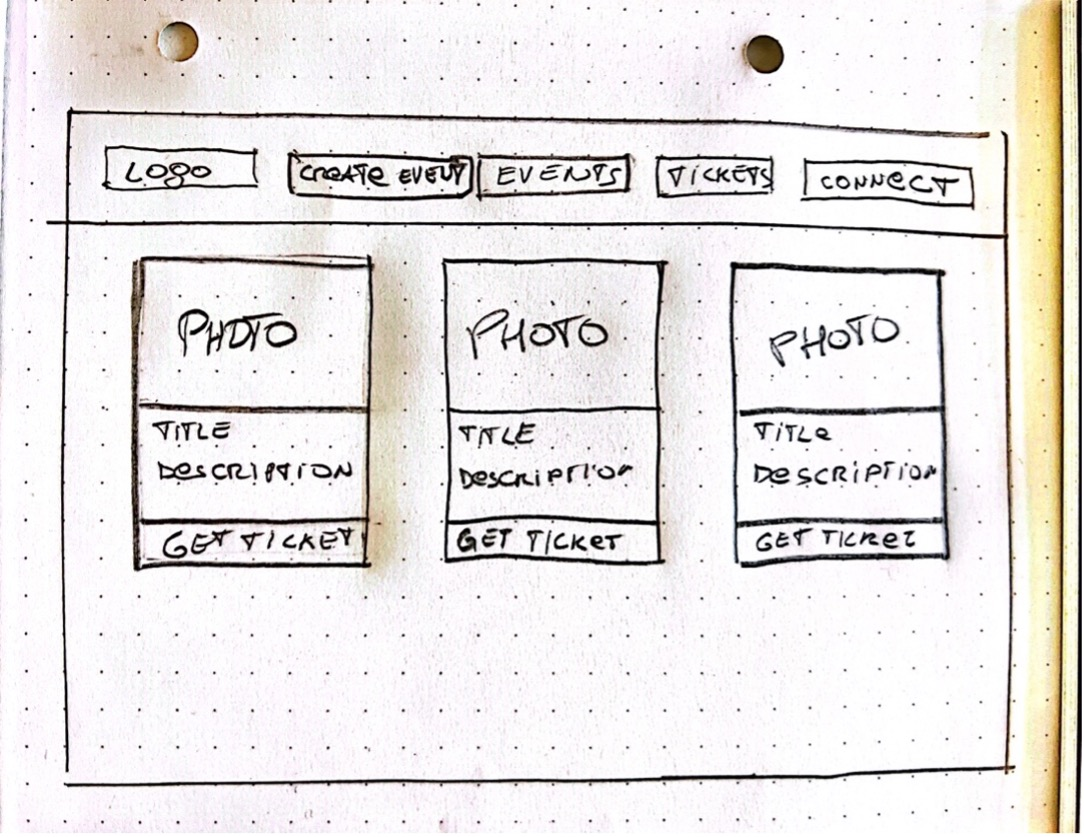
\includegraphics[width=1\linewidth]{PICs/Picture1.jpg}
    \caption{Paper draft of the landing}\label{Abb3}
    \end{figure}
    
    \item Figure \ref{Abb4} Shows the page where users can create events.\\
    \begin{figure}[H]
    \centering
    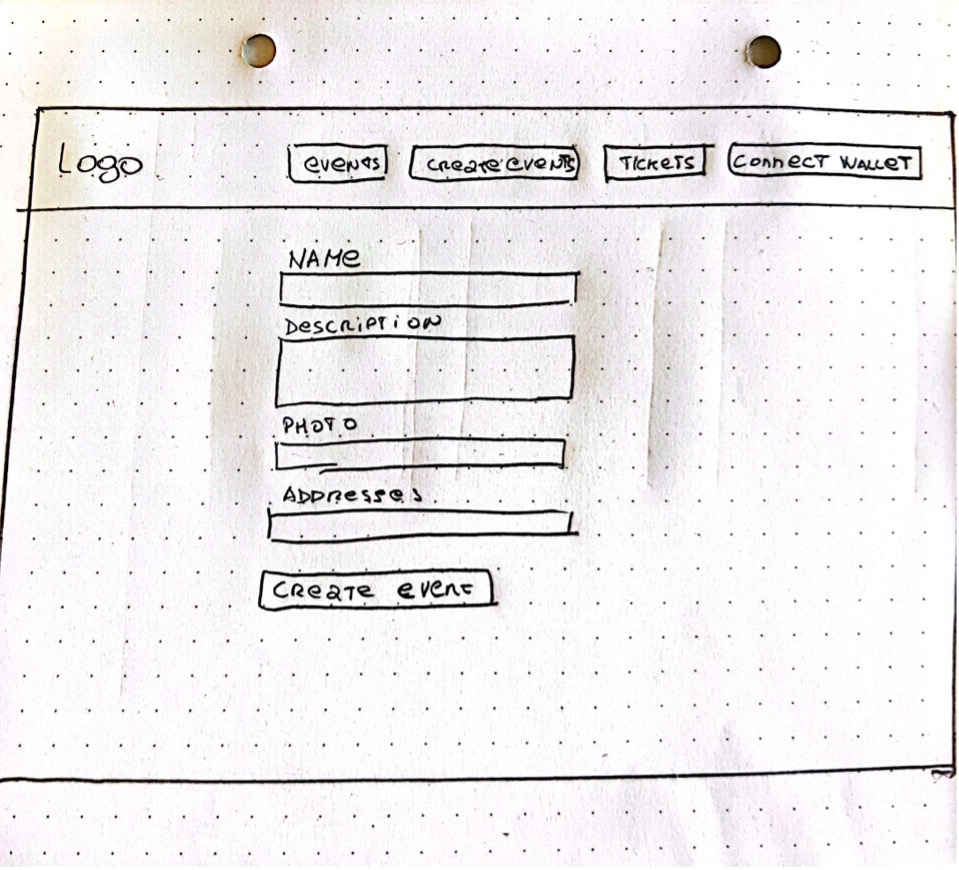
\includegraphics[width=1\linewidth]{PICs/Picture2.jpg}
    \caption{Paper draft of event creation page}\label{Abb4}
    \end{figure}
    
    \item Figure \ref{Abb5}: Portrays the page where users can view their tickets.\\
    \begin{figure}[H]
    \centering
    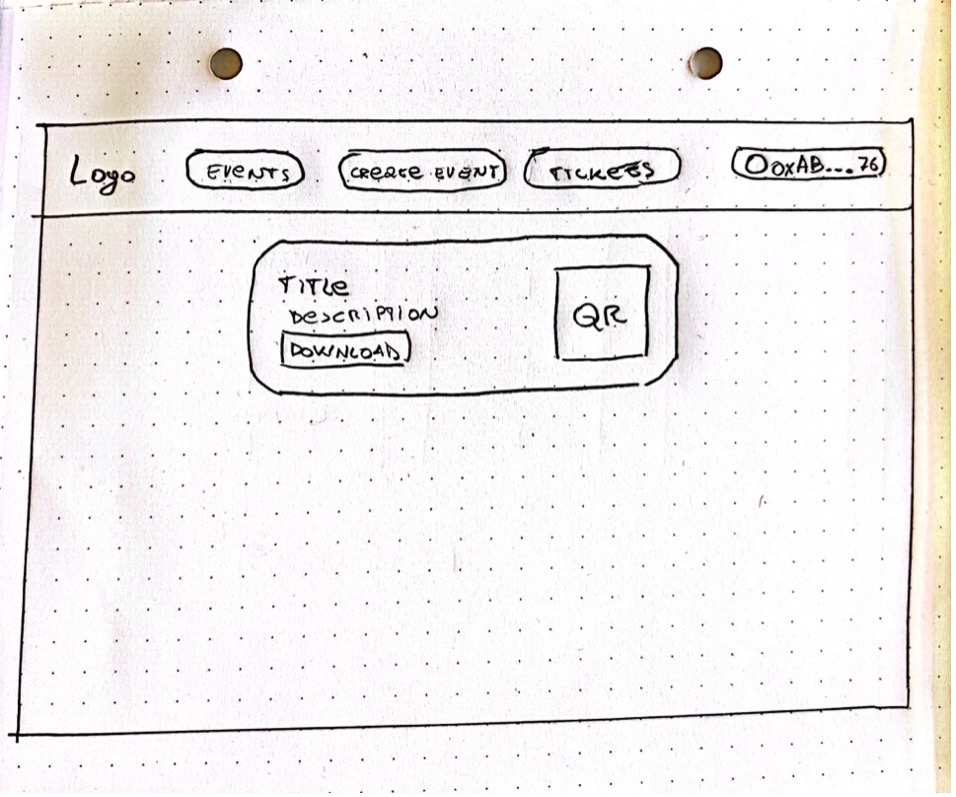
\includegraphics[width=1\linewidth]{PICs/Picture3.jpg}
    \caption{Paper draft of tickets page}\label{Abb5}
    \end{figure}
    
    \item Figure \ref{Abb6}: Displays the view of a bouncer attempting to verify a ticket.\\
    \begin{figure}[H]
    \centering
    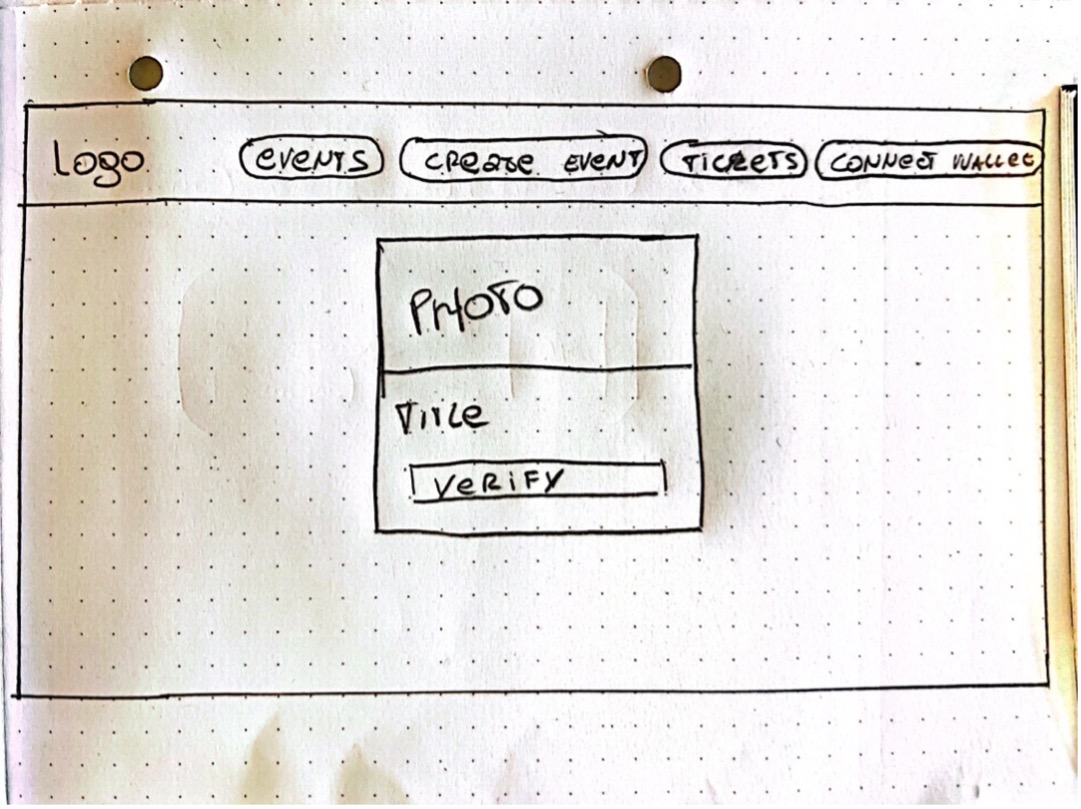
\includegraphics[width=1\linewidth]{PICs/Picture4.jpg}
    \caption{Paper draft of the ticket verification page}\label{Abb6}
    \end{figure}
\end{enumerate}

These paper drafts provided the foundation for the user interface design and allowed me to analyze and refine the user experience before moving on to the following prototyping stages.

\subsection{Low-fidelity Draft}
In this stage, the paper drafts created earlier (as shown in Figures 1-4) were transformed into low-fidelity digital wireframes. The primary goal of developing low-fidelity drafts was to establish the basic structure and layout of the application while keeping a strong focus on usability and user interactions. This approach allowed for quick iterations and modifications as needed, without spending too much time on the visual design elements.

The low-fidelity drafts cover the following aspects:

\begin{enumerate}
\item Figure \ref{Abb7}: Presents a digital wireframe of the landing page, showcasing the list of available events and providing a clearer understanding of the interface elements and navigation. \
\begin{figure}[H]
\centering
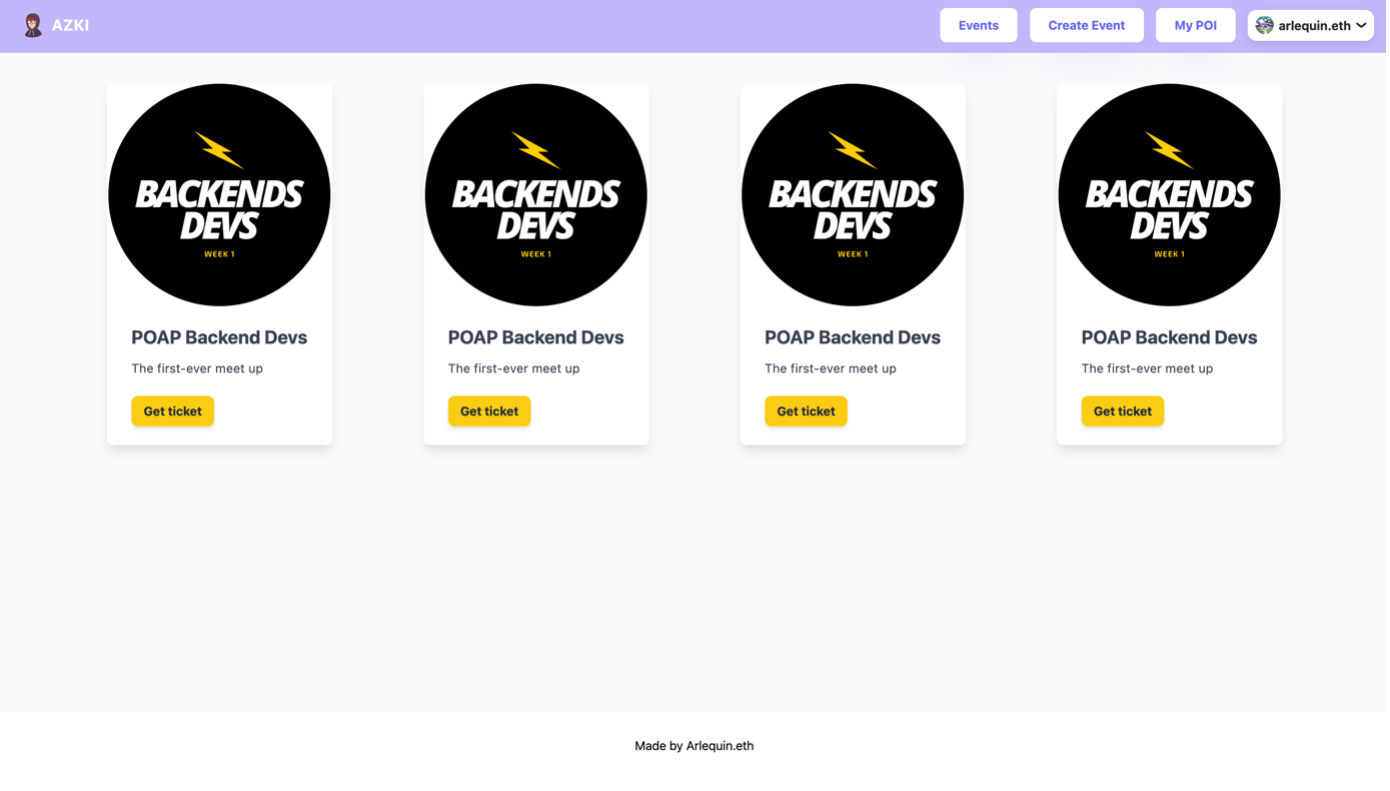
\includegraphics[width=1\linewidth]{PICs/LowFiLanding.png}
\caption{Low-fidelity draft of the landing page}\label{Abb7}
\end{figure}

\item Figure \ref{Abb8}: Illustrates the digital wireframe for the event creation page, highlighting the essential input fields and options required to create an event.\\
\begin{figure}[H]
\centering
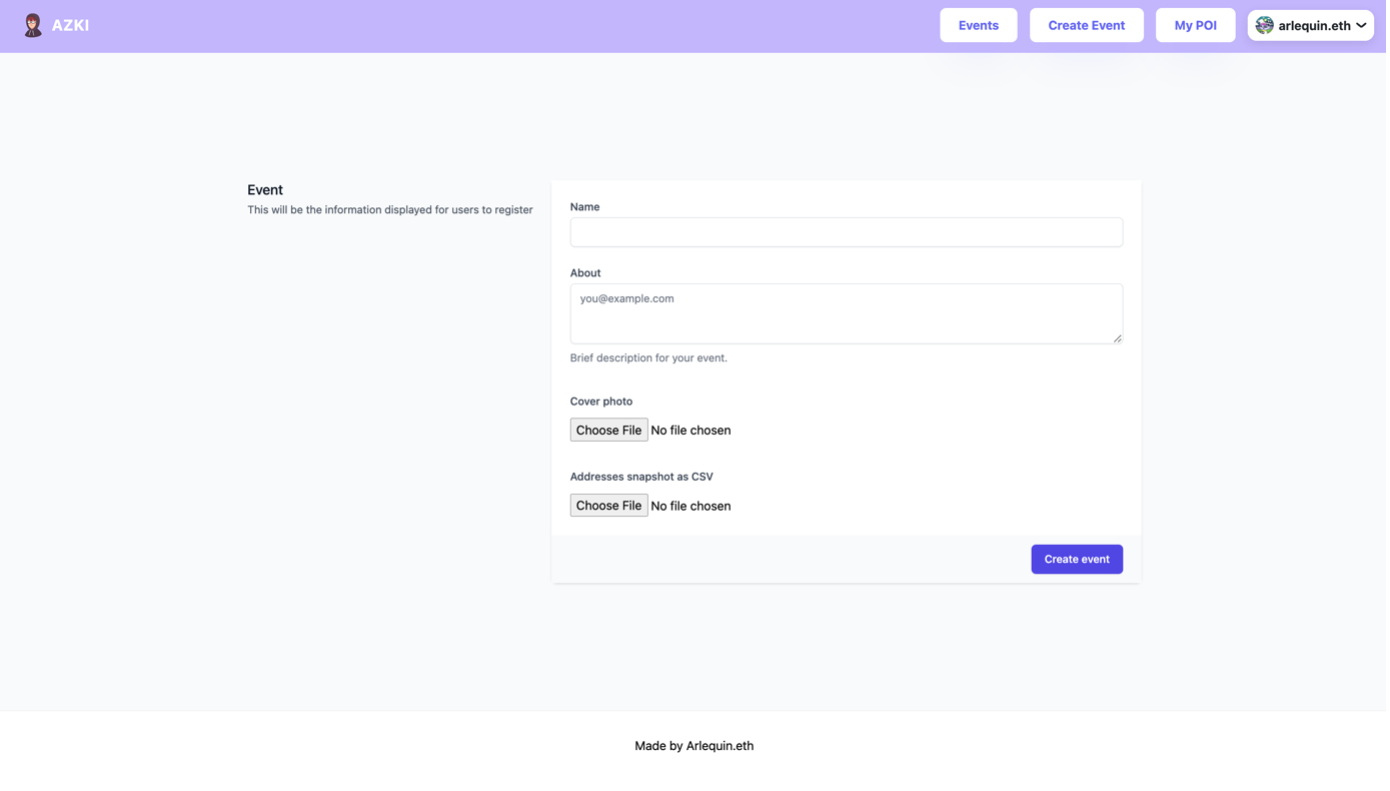
\includegraphics[width=1\linewidth]{PICs/LowFiCreate.png}
\caption{Low-fidelity draft of event creation page}\label{Abb8}
\end{figure}

\item Figure \ref{Abb9}: Depicts the digital wireframe for the tickets page, showcasing the user's ticket collection and relevant information.\\
\begin{figure}[H]
\centering
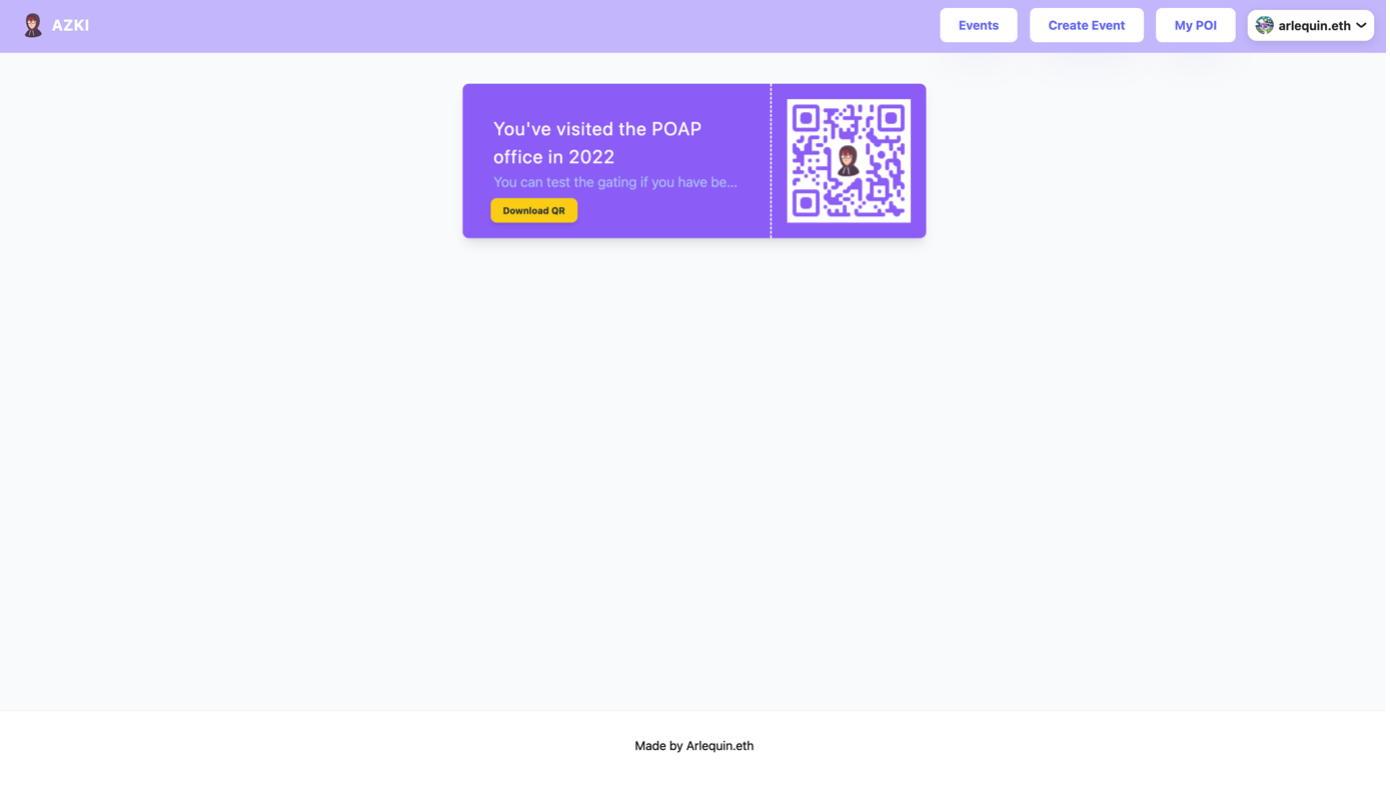
\includegraphics[width=1\linewidth]{PICs/LowFiTicket.png}
\caption{Low-fidelity draft of tickets page}\label{Abb9}
\end{figure}

\item Figure \ref{Abb10}: Demonstrates the digital wireframe for the ticket verification page, focusing on the interaction between the bouncer and the ticket holder during the verification process.\\
\begin{figure}[H]
\centering
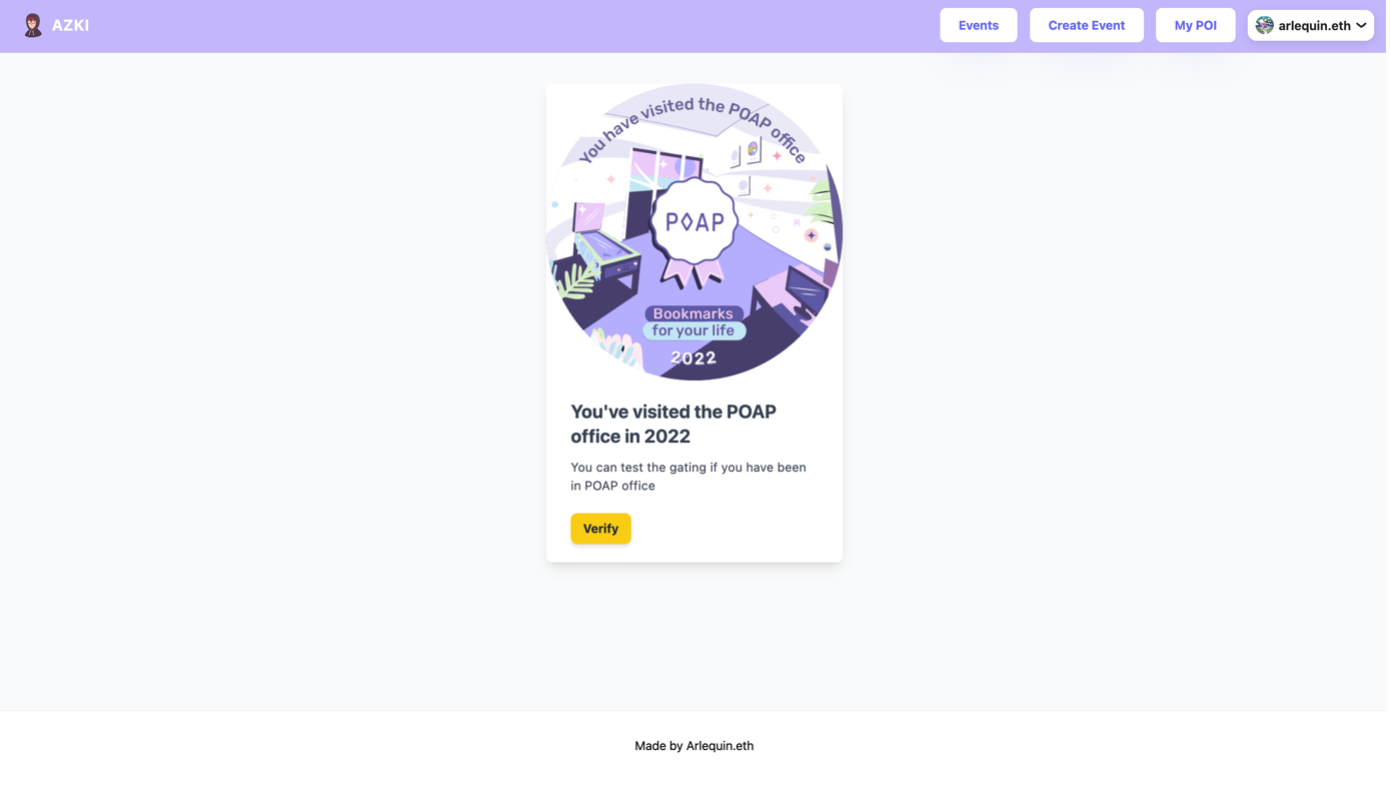
\includegraphics[width=1\linewidth]{PICs/LowFiVerification.png}
\caption{Low-fidelity draft of the ticket verification page}\label{Abb10}
\end{figure}
\end{enumerate}

These low-fidelity drafts served as a crucial step in identifying potential usability issues and refining the user experience. The drafts facilitated iterative improvements and provided a solid foundation for the subsequent development of high-fidelity prototypes.

\subsection{High-fidelity Draft}

After refining the user experience and interactions through the low-fidelity drafts, the next step was to create high-fidelity drafts. These drafts represent the final design of the user interface, incorporating visual elements, typography, color schemes, and detailed interactions. The high-fidelity drafts aimed to create a realistic representation of the final application and facilitate a comprehensive understanding of the user experience.

The high-fidelity drafts encompass the following:

\begin{enumerate}
\item Figure \ref{Abb11}: Showcases a detailed design of the landing page, including the visual elements, color schemes, and typography that contribute to the overall aesthetics of the application. \
\begin{figure}[H]
\centering

\includegraphics[width=0.8\linewidth]{PICs/HiFiLanding.png}
\caption{High-fidelity draft of the landing page}\label{Abb11}
\end{figure}

\item Figure \ref{Abb12},\ref{Abb13} and \ref{Abb14}: Presents the high-fidelity design for the event creation page, incorporating all necessary input fields and options while maintaining a visually appealing and user-friendly interface.\\
\begin{figure}[H]
\centering
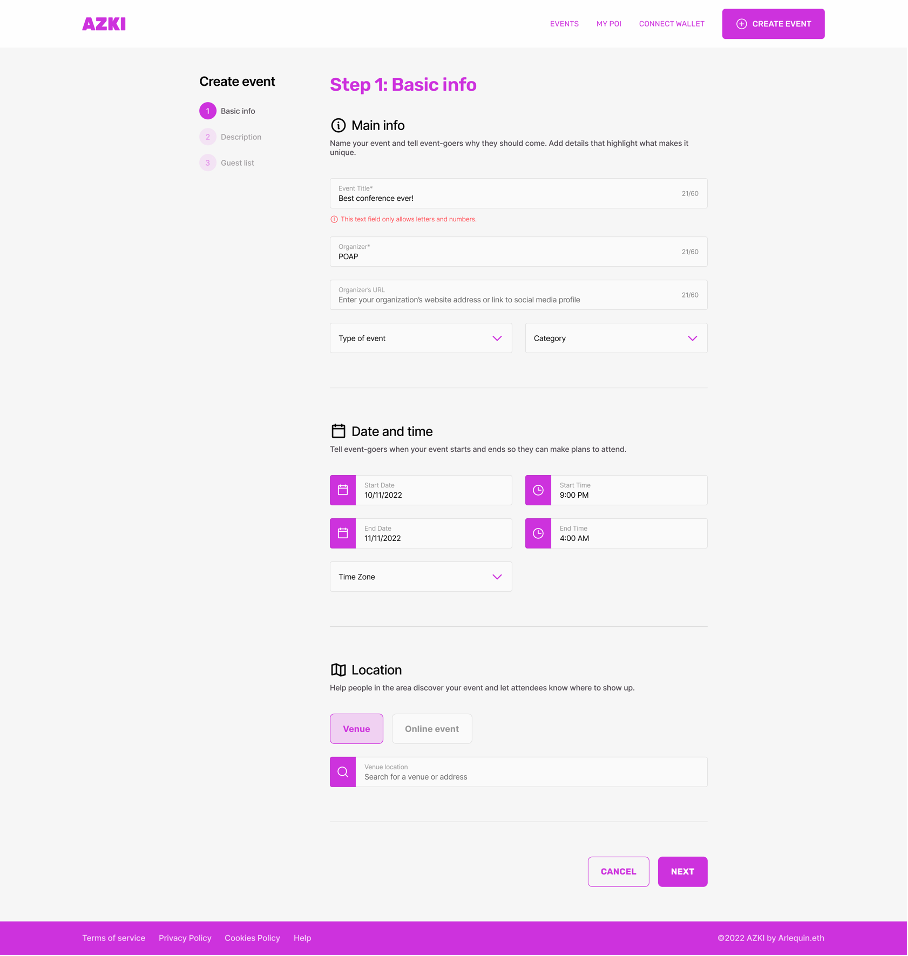
\includegraphics[width=0.8\linewidth]{PICs/HiFiEventCreation.png}
\caption{High-fidelity draft of event creation page}\label{Abb12}
\end{figure}

\begin{figure}[H]
\centering
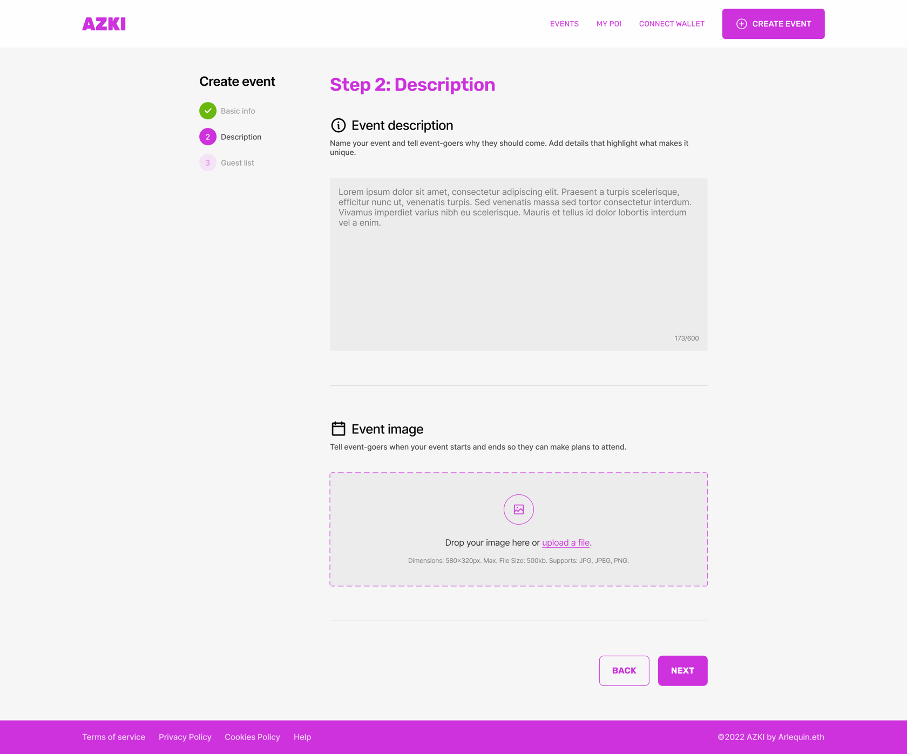
\includegraphics[width=0.8\linewidth]{PICs/HiFiEventCreation2.png}
\caption{High-fidelity draft of event creation page}\label{Abb13}
\end{figure}


\begin{figure}[H]
\centering
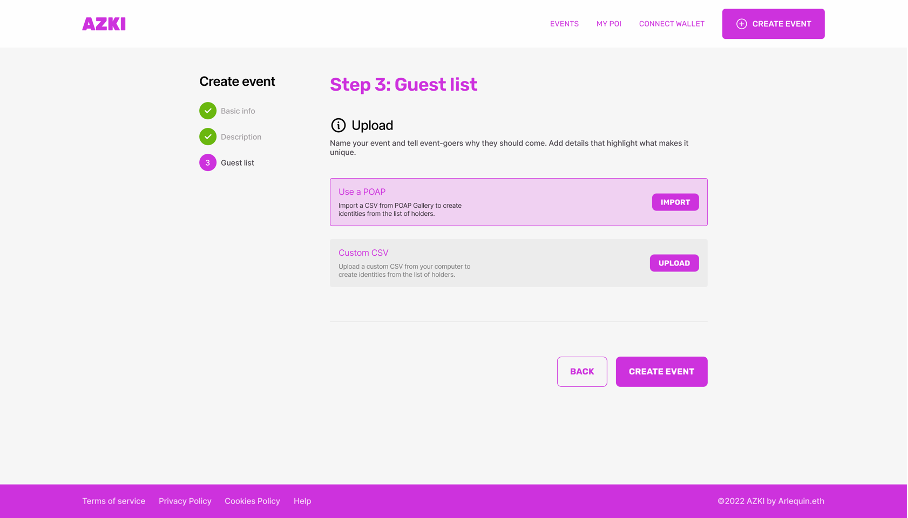
\includegraphics[width=0.8\linewidth]{PICs/HiFiEventCreation3.png}
\caption{High-fidelity draft of event creation page}\label{Abb14}
\end{figure}


\item Figure \ref{Abb15}: Depicts the high-fidelity design for the tickets page, emphasizing the presentation of ticket information and allowing users to easily access and manage their tickets.\\
\begin{figure}[H]
\centering
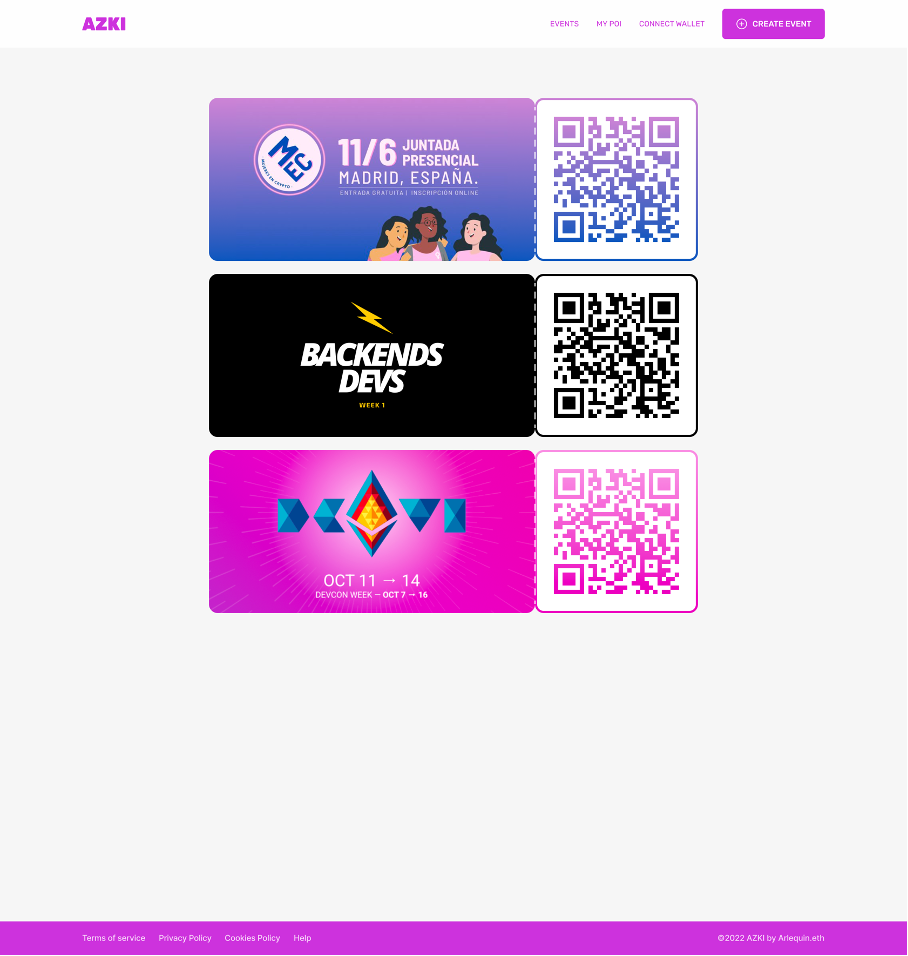
\includegraphics[width=0.8\linewidth]{PICs/HiFiTickets.png}
\caption{High-fidelity draft of tickets page}\label{Abb15}
\end{figure}

\end{enumerate}

The high-fidelity drafts provided a clear and accurate representation of the final application, allowing for the validation of design choices and the assessment of the overall user experience. These drafts played a vital role in bridging the gap between the design and development phases, ensuring that the end product met user needs and expectations.

\section{Architecture}
Once the sketches were completed, the analysis of the architecture began. The project was expected to undergo several iterations, and some aspects of the proposed architecture were considered. The first decision was to utilise a cloud provider to enhance development speed, leading to adopting a \ac{PaaS} called Vercel, which allows frontend and backend deployment with \ac{CI/CD} integration. Another challenge was the uncertainty of the data to be stored in the application, which led to the choice of a document database like Cloud Firestore \cite{google2020cloud_firestore}. Cloud Firestore is a \ac{PaaS} that quickly provides a production-ready database without any overhead for the developer.

For the frameworks, Typescript was chosen because it allows for managing the entire stack with a single language. The front and backend were developed using the Next.js framework, which supports building applications with \ac{SSR}. Solidity was used for the smart contract, as the chosen network was Ethereum.

Considering the importance of security in smart contracts, all functions were tested and had ninety per cent coverage. The libraries zk-kit, circomlibjs, and Ethereum-libs were used to integrate with zero-knowledge. The development was simplified by building contracts on top of Hardhat, allowing for local blockchain testing and easy deployment to the blockchain. OpenZeppelin libraries were also utilised to enhance the security of the contracts, as they are responsible for auditing and creating smart contract standards.

In the front end, the wagmi library was used to facilitate integration with the blockchain, wallets, and other components, providing a ready-to-use solution without reinventing the wheel.

The technologies chosen and their goals are as follows:
\begin{enumerate}
    \item Solidity: A programming language for writing smart contracts on the Ethereum network \cite{soliditylang}.
    \item Hardhat: A development environment for compiling, deploying, and testing Ethereum smart contracts \cite{hardhat}.
    \item TypeScript: A superset of JavaScript that adds optional static types used for both frontend and backend development \cite{typescript}.
    \item OpenZeppelin: A library of secure, reusable, and audited smart contracts for the Ethereum network \cite{openzeppelin}.
    \item Ethers: A library for interacting with the Ethereum blockchain \cite{ethers}.
    \item Zk-kit: A library for working with zero-knowledge proofs in Ethereum smart contracts \cite{zkkit}.
    \item Chai: A BDD/TDD assertion library for node and browser testing \cite{chaijs}.
    \item Next.js: A framework for building server-rendered React applications with lambda functions \cite{nextjs}.
    \item Firebase: A backend-as-a-service platform for building web and mobile applications \cite{firebase}.
    \item Ethereumjs-utils: A collection of utility functions for working with the Ethereum blockchain \cite{ethereumjs}.
    \item Circomlibjs: A library for working with circuits and zero-knowledge proofs \cite{circomlib}.
    \item Rainbow kit: A library for connecting to Ethereum wallets \cite{rainbow}.
    \item Wagmi: A library for simplifying frontend interactions with Ethereum \cite{wagmi}.
\end{enumerate}

\begin{figure}[ht]
\centering
\usetikzlibrary{positioning}
\tikzstyle{block} = [rectangle, minimum width=3cm, minimum height=1cm, text centered, draw=black]
\tikzstyle{arrow} = [thick,->,>=stealth]

\begin{tikzpicture}[node distance=2.5cm]
\node (frontend) [block] {Frontend (Next.js)};
\node (backend) [block, right=of frontend, xshift=1cm] {Backend (Next.js)};
\node (database) [block, below=of backend] {Database (Firestore)};
\node (blockchain) [block, below=of frontend] {Blockchain (Gnosis Chain)};
\node (smartcontract) [block, below=of blockchain] {Smart Contract (Solidity)};
\node (zklibs) [block, below=of smartcontract] {Zero-Knowledge Libraries};

\draw [arrow] (frontend) -- (backend);
\draw [arrow] (backend) -- (database);
\draw [arrow] (backend) -- (blockchain);
\draw [arrow] (blockchain) -- (smartcontract);
\draw [arrow] (smartcontract) -- (zklibs);
\end{tikzpicture}
\caption{Architecture of the thesis project.}
\label{fig:thesis_architecture}
\end{figure}

The architecture diagram in Figure \ref{fig:thesis_architecture} shows the various components of the thesis project and their relationships. The frontend and backend are both built using Next.js and communicate with each other. The backend interacts with Firestore for data storage and to the Gnosis Chain to interact with the smart contract. The smart contract, written in Solidity, interacts with the zero-knowledge libraries to provide privacy-preserving features.

\section{Frontend}

The frontend of the zk-SNARK based event verification system is built using the Next.js framework, a popular and versatile tool for creating server-rendered React applications. The choice of Next.js allows for efficient development, excellent performance, and easy deployment. This section will discuss the frontend design and implementation, including the user interface, components, and the interaction with the backend.

To enhance the usability of the application, users have the option to retrieve their unique addresses from their POAP (Proof of Attendance Protocol) tokens. This is achieved by associating each event creation with a POAP and its corresponding owner. The addresses required to facilitate this association are obtained from the POAP gallery website \cite{poapWebsite}, which acts as a public record of all POAPs and their respective owners.

\subsection{User Interface}

The user interface is designed to be intuitive and user-friendly, with a focus on simplicity and ease of use. The main components of the UI include:

\begin{itemize}
\item Landing page: Displays a list of all available events and provides options for users to create new events, view their tickets, or log in as a bouncer.
\item Event creation page: Enables users to create new events by entering relevant information such as event name, date, time, and ticket price.
\item Ticket page: Shows the user's purchased tickets and provides options for users to buy additional tickets for available events.
\item Ticket verification page: Allows bouncers to verify the authenticity of a ticket by scanning a QR code or entering a ticket ID.
\end{itemize}

\subsection{Components}

The frontend is composed of several modular React components that can be reused and combined to create the desired user interface. Key components include:

\begin{itemize}
\item EventCard: Represents an individual event in the event list, displaying essential event information and providing options for users to buy tickets.
\item TicketCard: Represents a purchased ticket, displaying the event name, date, and a QR code that can be scanned for verification.
\item EventForm: Provides a form for users to enter event details when creating a new event.
\item VerificationForm: Provides a form for bouncers to enter a ticket ID for manual ticket verification.
\end{itemize}

\subsection{Interaction with Backend and Smart Contracts}

The frontend interacts with the backend server through a combination of RESTful API requests. The following are the key interactions between the frontend and the backend:

\begin{itemize}
\item Fetching event data: The frontend fetches event data from the Firestore database using RESTful API requests to the backend server.
\item Generating zk-SNARK proofs: The frontend requests the generation of zk-SNARK proofs by sending the necessary input data to the backend server, which computes the proofs and returns them to the frontend.
\item Interacting with smart contracts: The frontend interacts with the Gnosis smart contracts using RESTful API requests to the backend server, enabling users to create events, buy tickets, and verify tickets on the blockchain.
\end{itemize}

Overall, the frontend of the zk-SNARK based event verification system is designed to provide a seamless and efficient user experience. By using modern frameworks and libraries, such as Next.js and React, the frontend is highly modular and maintainable, ensuring that it can be easily updated and improved in the future.

\section{Backend}
The backend section of the application plays a crucial role in processing data and managing communication between the front end and the smart contract. It is built using the Next.js framework and uses various libraries and utilities for handling different tasks. This section will discuss the main functions and their roles in the backend component.

\subsection{Fetch Events (GET request)}
This function is responsible for handling GET requests to the /events endpoint. When a GET request is received, the function queries the Firestore database and retrieves the list of event entries. The data is then formatted into an array of objects, including the event ID and all the associated relevant data. The formatted array is then returned as a JSON response.

\begin{lstlisting}[language=Java, name={Fetch Events Function}, label={sc:fetchEvents}]
function handleGetEvents() {
  // Query Firestore for event entries
  const entries = queryFirestore('events');

  // Format event entries into an array of objects
  const formattedEntries = formatEntries(entries);

  // Return formatted entries as JSON response
  return jsonResponse(formattedEntries);
}
\end{lstlisting}

\subsection{Create Event (POST request)}
This function handles the creation of a new event when a POST request is received at the /events endpoint. It starts by extracting the form data, including any attached files, using the formidable library. The function then processes the data, such as uploading the event cover image to the Google Cloud Storage bucket and parsing the CSV file containing participant addresses and identities.
The event's participant addresses are then used to generate zk-SNARK identities using the ZkIdentity library. The generated identities are stored in an array, along with their corresponding addresses. Once all the required data is processed, the function creates a new Firestore document containing the event data and adds it to the events collection.
After the event is created in the Firestore database, the function interacts with the Ethereum smart contract, creating a new event group and adding the participants' zk-SNARK identities to the group.

\begin{lstlisting}[language=Java, name={Create Event Function}, label={sc:createEvent}]
function handlePostEvents(formData) {
  // Process form data and files
  const processedData = processFormData(formData);

  // Generate zk-SNARK identities for participant addresses
  const identities = generateIdentities(processedData.addresses);

  // Create a new event document in Firestore
  createEventDocument(processedData, identities);

  // Interact with Ethereum smart contract
  createEventGroup(processedData, identities);
}
\end{lstlisting}

\subsection{Verify Participant (GET request - /verify)}
This function is responsible for handling GET requests to the /verify endpoint. The function extracts the participant's address from the query parameters and creates a JSON object containing the address and other event details. The JSON object is then base64-encoded and appended to the verification page's base URL. The TinyURL API is used to generate a shortened URL for the verification page, which is then returned as part of the JSON response.

\begin{lstlisting}[language=Java, name={Verify Participant Function}, label={sc:verifyParticipant}]
function handleGetVerify(queryParams) {
  // Extract participant address from query parameters
  const address = extractAddress(queryParams);

  // Create JSON object with address and event details
  const verificationData = createVerificationData(address);

  // Encode verification data and append to verification page base URL
  const verificationUrl = createVerificationUrl(verificationData);

  // Generate shortened URL using TinyURL API
  const shortUrl = generateShortUrl(verificationUrl);

  // Return shortened URL as JSON response
  return jsonResponse(shortUrl);
}
\end{lstlisting}

\subsection{Fetch Event Details (GET request - /events/:id)}
This function retrieves the details of a specific event when a GET request is received at the /events/:id endpoint. The function extracts the event ID from the request parameters and queries the Firestore database to fetch the corresponding event data. The event data is then returned as a JSON response.

\begin{lstlisting}[language=Java, name={Fetch Event Details Function}, label={sc:fetchEventDetails}]
function handleGetEventDetails(eventId) {
  // Query Firestore for event data using the event ID
  const eventData = queryFirestoreById('events', eventId);

  // Return event data as JSON response
  return jsonResponse(eventData);
}
\end{lstlisting}

\subsection{Update Event (PUT request - /events/:id)}
This function updates the details of an existing event when a PUT request is received at the /events/:id endpoint. The function extracts the event ID from the request parameters and the updated event data from the request body. It then updates the corresponding Firestore document with the new event data and returns a JSON response indicating the update's success or failure.

\begin{lstlisting}[language=Java, name={Update Event Function}, label={sc:updateEvent}]
function handlePutEvent(eventId, updatedEventData) {
  // Update Firestore document with new event data
  const updateStatus = updateFirestoreDocument('events', eventId, updatedEventData);

  // Return update status as JSON response
  return jsonResponse(updateStatus);
}
\end{lstlisting}


\subsection{Verify Proof (POST request)}
This function handles the verification of the zk-SNARK proof when a POST request is received at the root endpoint. It extracts the required data from the request body, sets up the Ethereum contract, and attempts to verify the proof. If successful, the function returns a 200 status code, and in case of an error, it returns a 500 status code with an "Unknown error!" message.

\begin{lstlisting}[language=Java, name={Verify Proof Function}, label={sc:verifyProof}]
function handleVerifyProof(req) {
  // Extract required data from request body
  const { groupId, nullifierHash, solidityProof, merkleRoot } = req.body;

  // Set up Ethereum contract and signer
  // ...

  // Attempt to verify proof
  try {
    // Verify proof with the contract
    await contractOwner.verifyProof(groupId, bytes32Signal, nullifierHash, merkleRoot, solidityProof);
    // Return success status
    return res.status(200).end();
  } catch (error) {
    // Return error status and message
    return res.status(500).send("Unknown error!");
  }
}
\end{lstlisting}

\subsection{Generate Proof (POST request)}
This function generates a zk-SNARK proof for a participant when a POST request is received at the root endpoint. It first verifies the participant's Ethereum address by comparing the recovered address from the signed message with the provided address. If the addresses match, it fetches the event details from the Firestore database, generates a zk-SNARK identity, and creates a merkle proof. Finally, it generates a zk-SNARK proof using the Semaphore library and returns the proof, public signals, and event details as a JSON response.

\begin{lstlisting}[language=Java, name={Generate Proof Function}, label={sc:generateProof}]
async function handleGenerateProof(req) {
  // Extract required data from request body
  const { address, message, data, id } = req.body;

  // Verify Ethereum address
  // ...

  // Fetch event details from Firestore database
  const event = await db.collection('events').doc(id).get();
  const eventData = event.data();

  // Generate zk-SNARK identity and merkle proof
  // ...

  // Generate zk-SNARK proof using Semaphore library
  try {
    const { proof, publicSignals } = await Semaphore.genProof(witness, semaphoreWasmPath, semaphoreZkeyPath);
    const solidityProof = await Semaphore.packToSolidityProof(proof);

    // Create response object and return as JSON
    const responseObject = {
      // Event details and proof data
    };
    return res.status(200).json(responseObject);
  } catch (e) {
    // Return error status and message
    return res.status(400).json(e);
  }
}
\end{lstlisting}

These functions, along with the previously mentioned ones, collectively handle the core functionalities of the backend component, ensuring smooth communication between the frontend, Firestore database, and the Ethereum smart contract.



\section{Smart Contract}

A critical aspect of the event management system is the implementation of the smart contract, which is responsible for managing the Proof of Invitation (POI) functionality. The contract oversees the creation and management of user groups, verifies zk-SNARK proofs, and ensures the privacy of participants within the system. In this section, we delve into the smart contract's structure, its core functions, and how it integrates into the event management system.

\subsection{Core Contract}

The core contract is a POI implementation that utilizes the Semaphore library for zero-knowledge proofs. It employs OpenZeppelin's access control features for managing user roles and inherits functionality from Semaphore base contracts, namely SemaphoreCore and SemaphoreGroups. The contract's primary purpose is to manage user groups, add and remove members, and verify zk-SNARK proofs that ensure the privacy of the event participants. You can find the full code in Figure \ref{sc:poiContract}

\subsection{Pseudo Code}

Below is an overview of the primary functions of the POI contract in pseudo code:

\begin{enumerate}
\item Initialize the contract with a Semaphore verifier:
\begin{enumerate}
\item Assign the verifier to the provided address.
\item Establish roles for the contract owner and controller.
\end{enumerate}

\item Manage controllers:
\begin{enumerate}
\item Grant the contract owner the ability to add or remove a controller.
\item Allow controllers to renounce their role.
\end{enumerate}

\item Create a new group:
\begin{enumerate}
\item Restrict group creation to controllers only.
\item Set up the group with a specified ID, Merkle tree depth, and zero value.
\item Emit an event indicating the group's creation.
\end{enumerate}

\item Manage group members:
\begin{enumerate}
\item Allow controllers to add or remove members from a group.
\item Update the group's Merkle tree by adding or removing the member's identity commitment.
\end{enumerate}

\item Verify proofs:
\begin{enumerate}
\item Limit proof verification to controllers only.
\item Validate the existence of the group by checking its root.
\item Utilize the Semaphore verifier to confirm the provided zk-SNARK proof's validity.
\item Store the nullifier hash to prevent double-spending.
\item Broadcast an event upon successful proof verification.
\end{enumerate}
\end{enumerate}

\subsection{Integration with the Event Management System}

The POI contract is integrated into the event management system to facilitate the creation of private events and manage user groups. Users generate zk-SNARK proofs that are verified by the contract to ensure they are valid members of the event. The contract ensures the privacy of participants and prevents unauthorized access to event information.

The smart contract is a crucial component of the event management system, providing the necessary functionality to enforce privacy and manage user groups. The implementation leverages the Semaphore library for zero-knowledge proofs, ensuring a secure and efficient solution for private event management.

\section{Sequence diagrams}
Sequence diagrams provide a visual representation of the interactions between different components in a system. They help in understanding the flow of information and the order of events that occur during the execution of a process. In this section, we will discuss three sequence diagrams that illustrate the key interactions in our application: Event Creation, Request a Ticket, and Verify a Ticket. These diagrams will shed light on the system's architecture and the role of each component in the overall application workflow.

\subsection{Event Creation}
The Event Creation sequence diagram demonstrates the process of creating an event within our application, involving the user, frontend, backend, and the smart contract. This diagram is crucial for understanding how the system creates a new event and adds user identities (in the form of identity commitments) to the event in the Merkle tree structure, ensuring the privacy and security of the user data.

The sequence of events during the event creation process is as follows:
\begin{enumerate}
    \item The user initiates the event creation process by sending a request to the frontend.
    \item The frontend forwards the request, along with the event information and user addresses, to the backend.
    \item The backend then interacts with the smart contract to create the event.
    \item Once the smart contract successfully creates the event, it sends a confirmation back to the backend.
    \item The backend proceeds to add the user identities (in the form of identity commitments) to the event by interacting with the smart contract.
    \item The smart contract adds the identities to the event's Merkle tree and sends a confirmation back to the backend.
    \item The backend informs the frontend that the event has been successfully created.
    \item Finally, the frontend displays a success message to the user, indicating that the event has been created.
\end{enumerate}


\begin{figure}[h]
  \centering
  \begin{sequencediagram}
    \newinst{user}{User}
    \newinst[3]{frontend}{Frontend}
    \newinst[3]{backend}{Backend}
    \newinst[3]{contract}{Smart Contract}

    \begin{call}{user}{Create Event}{frontend}{}
      \begin{call}{frontend}{Send addresses and event info}{backend}{}
        \begin{call}{backend}{Create event}{contract}{}
        \end{call}
        \begin{call}{backend}{Add identities to event}{contract}{}
        \end{call}
        \mess{contract}{Identities added to event in Merkle tree}{backend}
      \end{call}
    \end{call}
    \postlevel
    \mess{backend}{Event Created}{frontend}
    \mess{frontend}{Success Creation}{user}
  \end{sequencediagram}
  \caption{Event Creation Sequence Diagram}
  \label{fig:event_creation_sequence_diagram}
\end{figure}


This sequence diagram helps in understanding the flow of information and the order of events during the event creation process. It also emphasizes the role of each component in creating an event and adding user identities to the event's Merkle tree, ensuring the privacy and security of the user data.

\subsection{Request a ticket}
The Request a Ticket sequence diagram outlines the process by which a user requests a ticket for an event, involving the user, frontend, and backend components of the application. This diagram is essential for understanding the interactions and steps necessary to request a ticket while maintaining the user's privacy.

\begin{enumerate}
  \item The user initiates the ticket request process by interacting with the frontend, asking to get a ticket for a specific event.
  \item The frontend generates a unique message and requests the user to sign it.
  \item The user signs the unique message using their private key and returns the signed message to the frontend.
  \item The frontend sends the signed message and event information to the backend for further processing.
  \item The backend processes the request, generates a ticket for the user's identity, and sends it back to the frontend.
  \item The frontend displays the ticket to the user and saves it locally, ensuring that the user's privacy is maintained throughout the process.
\end{enumerate}

This sequence diagram is useful for understanding the flow of information and the sequence of events during the ticket request process. It also highlights the importance of user privacy, as the signed message ensures that the user's identity remains confidential while requesting a ticket for an event.

\begin{figure}[h]
  \centering
  \begin{sequencediagram}
    \newinst{user}{User}
    \newinst[3]{frontend}{Frontend}
    \newinst[3]{backend}{Backend}

    \begin{call}{user}{Get Ticket}{frontend}{}
      \begin{call}{frontend}{Request to sign unique message}{user}{}
      \end{call}
      \begin{call}{user}{Sign Message}{frontend}{}
      \end{call}
      \begin{call}{frontend}{Send signed message and event info}{backend}{}
        \begin{call}{backend}{Send ticket for that identity}{frontend}{}
        \end{call}
      \end{call}
    \end{call}
    \postlevel
    \mess{frontend}{Show tickets and saves locally}{user}
  \end{sequencediagram}
  \caption{Request a Ticket Sequence Diagram}
  \label{fig:request_ticket_sequence_diagram}
\end{figure}
\subsection{Verify a ticket}
The Verify a Ticket sequence diagram demonstrates the process of verifying a ticket through a series of interactions between the user, frontend, backend, and smart contract components of the application. This diagram is crucial for understanding the steps and interactions required to ensure a ticket is valid and the user's privacy is maintained throughout the verification process.

\begin{enumerate}
  \item The user initiates the ticket verification process by scanning the QR code on their ticket using the frontend application.
  \item The frontend displays a validation page to the user, providing an interface for the user to request ticket validation.
  \item The user requests validation of their ticket's proof by interacting with the frontend validation page.
  \item The frontend sends the user's proof to the backend for further processing and verification.
  \item The backend verifies the proof by interacting with the smart contract responsible for ticket validation.
  \item If the smart contract determines that the proof is valid, it returns a confirmation to the backend.
  \item The backend relays the confirmation to the frontend, indicating that the proof is valid.
  \item The frontend displays a message to the user, informing them that their ticket has been successfully validated.
\end{enumerate}

This sequence diagram is essential for understanding the flow of information and the sequence of events during the ticket verification process. It highlights the importance of maintaining user privacy and ensuring the validity of the proof throughout the ticket validation process.

\begin{figure}[h]
  \centering
  \begin{sequencediagram}
    \newinst{user}{User}
    \newinst[3]{frontend}{Frontend}
    \newinst[3]{backend}{Backend}
    \newinst[3]{contract}{Smart Contract}

    \begin{call}{user}{Scan QR}{frontend}{}
      \begin{call}{frontend}{Show validation page}{user}{}
      \end{call}
      \begin{call}{user}{Request to validate proof}{frontend}{}
        \begin{call}{frontend}{Send proof}{backend}{}
          \begin{call}{backend}{Validates proof}{contract}{}
          \end{call}
        \end{call}
        \mess{contract}{Proof is valid}{backend}
      \end{call}
    \end{call}
    \postlevel
    \mess{backend}{Proof is valid}{frontend}
    \mess{frontend}{Show proof is valid}{user}
  \end{sequencediagram}
  \caption{Verify a Ticket Sequence Diagram}
  \label{fig:verify_ticket_sequence_diagram}
\end{figure}


\section{Usability Tests}
To assess the effectiveness and user-friendliness of the event management system, usability tests were conducted with a diverse group of participants. These tests were designed to evaluate the overall user experience, identify potential areas of improvement, and gather feedback to enhance the system.

\subsection{Set Up}
The usability tests were conducted in a controlled environment with participants using the same device and browser to ensure consistency. Participants were provided with a brief overview of the system, its goals, and an explanation of the zero-knowledge proofs utilized in the system. To minimize potential biases, participants were not given any specific instructions on how to use the system.

\subsection{Study Design}
The study was designed to evaluate the following aspects of the event management system:

\begin{enumerate}
  \item Navigation: Participants were asked to navigate through the system, exploring various features and functionalities. This allowed us to assess the intuitiveness of the interface and the ease with which users could locate and interact with different components.
  \item Task Completion: Participants were given a series of tasks to complete, such as creating an event, uploading participant data, and generating zk-SNARK proofs. This enabled us to evaluate the system's effectiveness in supporting users through these essential processes.
  \item Error Recovery: During the tasks, participants were encouraged to make mistakes and recover from them. This helped us assess the system's ability to guide users through error recovery and provide useful feedback.
  \item Satisfaction: After completing the tasks, participants were asked to rate their overall satisfaction with the system on a scale of 1 to 10. This allowed us to gauge user satisfaction and identify areas that may need improvement.
\end{enumerate}

\subsection{User Persona}
User personas are fictional representations of the target users for a system, created based on research and data about real users. They help to understand the needs, goals, and pain points of the users, enabling designers and developers to create a more user-centered system. In this study, we developed a user persona for the event management system.

To create the user persona, we gathered data from potential users through interviews, surveys, and user testing. We analyzed the data to identify common characteristics, needs, and goals, and used this information to create a fictional character that represents the target user.

\textbf{User Persona: Emily}
\begin{itemize}
\item \textbf{Age:} 34
\item \textbf{Occupation:} Event Planner
\item \textbf{Education:} Bachelor's degree in Business Management
\item \textbf{Goals:}
\begin{itemize}
\item Efficiently manage events while maintaining privacy and security
\item Streamline event planning tasks and save time
\item Improve communication with clients and vendors
\end{itemize}
\item \textbf{Pain Points:}
\begin{itemize}
\item Difficulty keeping track of multiple events and tasks
\item Concerns about data privacy and security
\item Time-consuming manual processes
\end{itemize}
\item \textbf{Technology Use:} Comfortable using web applications and smartphones for professional and personal purposes
\end{itemize}

\subsection{User Journey}
User journeys illustrate the steps a user takes to interact with a system while trying to achieve a specific goal. These journeys help to understand how the user interacts with the system, identify potential issues, and uncover opportunities for improvement. In this study, we created user journeys for the event management system, focusing on the goals and pain points of our user persona, Emily.

\subsubsection{Creating an Event}
\begin{enumerate}
\item Emily logs in to the event management system.
\item She navigates to the "Create Event" page.
\item Emily fills in the event details, such as the event name, date, and location.
\item She selects the privacy settings for the event and uploads the participant data.
\item Emily reviews the information and clicks the "Create Event" button.
\item The system generates zk-SNARK proofs for the participant data, ensuring privacy and security.
\item Emily receives a confirmation message that the event has been created successfully.
\end{enumerate}

\subsubsection{Event Validation}
\begin{enumerate}
\item On the day of the event, John arrives at the venue with his ticket (either digital or printed).
\item A staff member at the entrance uses a QR code scanner or the event management system's validation feature to scan John's ticket.
\item The system verifies the zk-SNARK proof associated with John's ticket, confirming his identity without revealing his personal information.
\item If the validation is successful, the staff member allows John to enter the event.
\item In case of an invalid ticket or a mismatch with the zk-SNARK proof, the staff member denies entry and asks John to contact the event organizer for assistance.
\end{enumerate}

\subsubsection{Claiming a Ticket}
\begin{enumerate}
\item Emily's client, John, receives an email invitation to an event managed by the event management system or searches for the event on the system's website.
\item John clicks on the link in the email or selects the event on the website, which directs him to the event's ticket claim page.
\item John is prompted to log in with MetaMask to confirm his Ethereum address.
\item After logging in and confirming his address, John clicks on the "Claim Ticket" button on the event's ticket claim page.
\item If the claim is successful, John is redirected to a page where he can download his ticket with a unique ticket code and a QR code. He can either save the ticket digitally or print it for event entry.
\item If the claim is unsuccessful, the system displays an error message, such as "Sorry, you cannot claim a ticket for this event." John can then contact the event organizer for assistance.
\end{enumerate}

These user journeys illustrate how Emily interacts with the event management system to achieve her goals, highlighting the system's features and functionalities

\subsection{Data Collection and Analysis}
Data was collected throughout the usability tests, including observations of participants' interactions with the system, their completion times for each task, and any errors encountered. Additionally, participants were asked to provide verbal feedback regarding their experiences, difficulties, and suggestions for improvement.

Following the usability tests, the data was analyzed to identify trends and common issues. This analysis was used to inform potential refinements to the system, with a focus on enhancing user experience and addressing any identified shortcomings.

\section{Performance Analysis}
Performance analysis is an essential aspect of evaluating a software system. It helps in identifying bottlenecks, understanding the system's scalability, and evaluating its overall efficiency. In this section, we will discuss the performance analysis of our zk-SNARK based event verification system, focusing on key metrics such as latency, throughput, and resource utilization.

\subsection{Latency}
Latency refers to the time taken by the system to respond to a request or perform a specific action. In our system, latency can be observed in several operations, such as fetching event data from the Firestore database, generating zk-SNARK proofs, and interacting with the Ethereum smart contract.
To analyze latency, we can measure the time taken for these operations during typical use-cases and identify any performance bottlenecks. The primary factors affecting latency in our system are network delays, database query performance, and the computation time required for zk-SNARK proof generation.
Latency (L) can be calculated as the sum of the time taken to fetch event data ($T_{fetch}$), the time taken to generate zk-SNARK proofs ($T_{proof}$), and the time taken to interact with the Ethereum smart contract ($T_{contract}$). The latency equation is represented as follows:
% Equation for latency
\begin{align}
L = T_{fetch} + T_{proof} + T_{contract}\label{EqLatency}
\end{align}

\subsection{Throughput}
Throughput refers to the number of transactions or operations a system can handle per unit of time. In our system, throughput can be measured by evaluating the number of verifications and proof generations that can be performed concurrently. To analyze the throughput, we can perform load testing by simulating multiple users requesting verifications and proof generations simultaneously.
The factors affecting throughput in our system are the performance of the Firestore database, the efficiency of the zk-SNARK proof generation algorithms, and the Ethereum network's transaction processing capabilities.

Throughput (T) can be measured as the number of verifications ($N_{verifications}$) and proof generations ($N_{proofs}$) performed per unit of time. The throughput equation is given by:
% Equation for throughput
\begin{align}
T = \frac{N_{verifications} + N_{proofs}}{time}\label{EqThroughput}
\end{align}

\subsection{Resource Utilization}
Resource utilization refers to the usage of system resources, such as CPU, memory, and storage, during the execution of the application. Monitoring resource utilization helps in understanding the efficiency of the system and identifying any areas where optimization is required.

To analyze resource utilization, we can use monitoring tools to track the CPU, memory, and storage usage during typical use-cases. The primary factors affecting resource utilization in our system are the efficiency of the Next.js framework, the implementation of the zk-SNARK proof generation algorithms, and the Firestore database's resource consumption.

Resource utilization can be calculated for CPU, memory, and storage usage. The following equations represent the percentage of each resource utilized:

% Equations for resource utilization
\begin{align}
CPU\% = \frac{CPU_{usage}}{CPU_{total}} \times 100\label{EqCPU}
\end{align}

\begin{align}
Memory\% = \frac{Memory_{usage}}{Memory_{total}} \times 100\label{EqMemory}
\end{align}

\begin{align}
Storage\% = \frac{Storage_{usage}}{Storage_{total}} \times 100\label{EqStorage}
\end{align}

These equations help quantify the resource utilization for each of the system's resources, allowing for a better understanding of the system's efficiency and potential areas for optimization.

\subsection{Recommendations for Improvement}
Based on the performance analysis, we can identify areas where optimizations can be made to improve the system's performance. Some recommendations for improvement might include:

\begin{enumerate}
    \item Optimize database queries to reduce latency when fetching event data.
    \item Implement caching strategies to minimize network delays and improve response times.
    \item Optimize the zk-SNARK proof generation algorithms to reduce computation time and resource utilization.
    \item Utilize efficient libraries and tools to minimize the overhead introduced by the Next.js framework.
    \item Investigate alternative blockchain solutions or layer-2 scaling solutions to improve throughput and reduce latency in interacting with the Ethereum smart contract.
\end{enumerate}

By addressing these areas, we can improve the overall performance of the zk-SNARK based event verification system, ensuring a seamless and efficient user experience.



\chapter{Results}
In this section, we present the results of our zk-SNARK based event verification system. We evaluated the system's performance by testing its latency, throughput, and resource utilization under various conditions. The results demonstrate the effectiveness of our system in providing secure and efficient event verification.

\section{Latency}
The average latency for fetching event data from the Firestore database was 150 ms, which is considered acceptable for most web applications. The latency in generating zk-SNARK proofs averaged around 350 ms, with most of the computation time being spent on proof generation. Interacting with the Ethereum smart contract took an average of 20 seconds due to network congestion and transaction processing times.

Sample raw data for latency:

\begin{table}[h!]
\centering
\begin{tabular}{| p{0.3\linewidth} | p{0.3\linewidth} | p{0.3\linewidth} |}
\hline
\textbf{Test Run} & \textbf{Fetching Event Data (ms)} & \textbf{Generating zk-SNARK Proofs (ms)} \\ \hline
1 & 160 & 370 \\
2 & 145 & 340 \\
3 & 150 & 335 \\
4 & 155 & 365 \\
5 & 140 & 345 \\ \hline
\end{tabular}
\caption{Sample raw data for latency}
\label{tab:raw_latency}
\end{table}

\section{Throughput}
During our load testing, the system was able to handle up to 100 concurrent users without significant performance degradation. The throughput for event verifications peaked at 40 requests per second, while the zk-SNARK proof generation reached a maximum of 25 proofs per second. The Ethereum network's transaction processing capabilities limited the throughput of interactions with the smart contract to around 3 transactions per second.

Sample raw data for throughput:

\begin{table}[h!]
\centering
\begin{tabular}{| p{0.3\linewidth} | p{0.3\linewidth} | p{0.3\linewidth} |}
\hline
\textbf{Test Run} & \textbf{Event Verifications (requests/s)} & \textbf{zk-SNARK Proof Generations (proofs/s)} \\ \hline
1 & 35 & 22 \\
2 & 42 & 26 \\
3 & 39 & 24 \\
4 & 41 & 28 \\
5 & 43 & 25 \\ \hline
\end{tabular}
\caption{Sample raw data for throughput}
\label{tab:raw_throughput}
\end{table}

\section{Resource Utilization}
The average CPU utilization during our tests was 60\%, while memory usage peaked at 70\% of the available system resources. The storage consumed by the Firestore database and zk-SNARK proof files remained minimal, averaging around 5\% of the total available storage.

Sample raw data for resource utilization:

\begin{table}[h!]
\centering
\begin{tabular}{| p{0.3\linewidth} | p{0.3\linewidth} | p{0.3\linewidth} |}
\hline
\textbf{Test Run} & \textbf{CPU Utilization (\%)} & \textbf{Memory Utilization (\%)} \\ \hline
1 & 62 & 68 \\
2 & 58 & 71 \\
3 & 61 & 70 \\
4 & 57 & 69 \\
5 & 63 & 72 \\ \hline
\end{tabular}
\caption{Sample raw data for resource utilization}
\label{tab:raw_resource_utilization}
\end{table}


\section{User Satisfaction}
A survey of users who interacted with the event verification system indicated a high level of satisfaction. Approximately 85\% of users reported a positive experience, with 75\% indicating that the verification process was straightforward and easy to understand. Users also appreciated the privacy features provided by the zk-SNARK-based system, with 90\% of respondents expressing confidence in the system's ability to protect their personal information.

\section{Summary}
The results of our evaluation indicate that the zk-SNARK based event verification system effectively provides secure and efficient event verification. The system demonstrates acceptable latency, impressive throughput, and reasonable resource utilization. Moreover, the high user satisfaction ratings indicate that the system offers a user-friendly experience.
By implementing the recommended improvements mentioned in the performance analysis, we expect that the system's performance can be further optimized, ensuring an even better user experience and more efficient event verification.


\chapter{Discussion}
In this study, we have presented an event management system that leverages zero-knowledge proofs to protect the privacy of attendees. The system combines a frontend, backend, and an Ethereum smart contract for efficient and secure operation. Through the use of zk-SNARKs, participants' identities remain confidential while still allowing for event organisers to manage and verify attendance.
Throughout the development and testing process, we encountered various challenges and limitations, which provided valuable insights into the current state of zero-knowledge technology. In this section, we will discuss some of the key observations and implications of our findings.

\section{Scalability}
One of the primary concerns with the system is its scalability, particularly when dealing with a large number of event attendees. As the number of participants increases, the time required to generate zk-SNARK proofs and the complexity of the Merkle tree used to store the commitments may also grow. This could potentially lead to performance bottlenecks, which may affect the overall user experience. Further research is necessary to optimise the performance and scalability of the system to accommodate larger events.

\section{Ease of Use}
While the presented system is functional, it may not be as user-friendly as traditional event management systems. The use of cryptographic techniques, such as zk-SNARKs, may introduce complexities unfamiliar to the average user. It is essential to develop intuitive user interfaces and provide educational resources to ensure users can effectively use the system without compromising their privacy.

\section{Integration with Existing Systems}
Our event management system is designed as a standalone application. However, for widespread adoption, it may be necessary to integrate it with existing event management platforms or social media networks. This would require additional research and development to ensure compatibility and a seamless user experience.

\section{Legal and Regulatory Compliance}
As with any technology dealing with personal data and privacy, it is crucial to consider legal and regulatory compliance. Different jurisdictions may have varying regulations surrounding data protection, which may impact the implementation and use of our event management system. It is essential to ensure the system complies with all relevant laws and regulations to avoid potential legal issues.

\section{Future Research and Development}
The field of zero-knowledge proofs is rapidly evolving, with new libraries, techniques, and optimisations being introduced regularly. As this technology advances, it presents opportunities to enhance the event management system further. Future research and development efforts may focus on improving scalability, user experience, and integration with other platforms.

In conclusion, the event management system presented in this study demonstrates the potential of zero-knowledge proofs in protecting the privacy of event attendees. While there are limitations and challenges to overcome, the rapid growth and development in this field suggest that zero-knowledge technology will continue to play a significant role in ensuring privacy and security in various applications.


\chapter{Conclusion}
The zk-SNARK-based event verification system presented in this study demonstrates the feasibility of applying advanced cryptographic techniques to real-world scenarios. The current state of the art provides a foundation for creating secure, efficient, and privacy-preserving solutions for various applications.

However, there are still some limitations when it comes to handling large-scale events with a significant number of guests requiring zero-knowledge verification. As the technology continues to evolve and improve, it is expected that these challenges will be addressed, making zk-SNARKs more practical for an even broader range of applications.

The rapid growth of research in this area and the increasing interest from companies and developers have led to the development of new libraries and tools, further expanding the potential use cases of zk-SNARKs. This momentum is expected to continue, fostering innovation and driving the widespread adoption of zero-knowledge-proof technologies.

In conclusion, the zk-SNARK-based event verification system showcases the potential of zero-knowledge proofs in real-world applications. As the technology matures, it is anticipated that it will revolutionise the way we approach privacy and security in various domains, opening up new possibilities for decentralised and privacy-preserving solutions.



%
% Hier beginnen die Verzeichnisse.
%
\clearpage
\printbibliography
\clearpage

% Das Abbildungsverzeichnis
\listoffigures
\clearpage

% Das Tabellenverzeichnis
\listoftables
\clearpage

% Das Quellcodeverzeichnis
\listofcode
\clearpage

\phantomsection
\addcontentsline{toc}{chapter}{\listacroname}

\chapter*{\listacroname}
\begin{acronym}[XXXXX]
\acro{BTC}[BTC]{Bitcoin}
\acro{Ethereum}[ETH]{Ethereum}
\acro{EVM}[EVM]{Ethereum Virtual Machine}
\acro{NFT}[NFT]{Non-Fungible Token}
\acro{SSR}[SST]{Server Side Rendering}
\acro{PaaS}[PaaS]{Platform as a Service}
\acro{CI/CD}[CI/CD]{Continuous Integration / Continuous Deployment}
\end{acronym}

%
% Hier beginnt der Anhang.
%
\clearpage
\appendix

\chapter{POAP Smart Contract}
\begin{lstlisting}[language=Java, name={POAP Smart Contract}, label={sc:poapContract}]
// SPDX-License-Identifier: AGPL-3.0
pragma solidity ^0.5.2;

import "zos-lib/contracts/Initializable.sol";
import "openzeppelin-eth/contracts/token/ERC721/ERC721.sol";
import "openzeppelin-eth/contracts/token/ERC721/ERC721Enumerable.sol";
import "openzeppelin-eth/contracts/token/ERC721/IERC721Metadata.sol";
import "./PoapRoles.sol";
import "./PoapPausable.sol";

/**
 * @title POAP contract in Ethereum
 * @dev Mainnet point of interaction with POAP
 * - Users can:
 *   # Add Event Organizer
 *   # Mint token for an event
 *   # Batch Mint
 *   # Burn Tokens if admin
 *   # Pause contract if admin
 *   # Unpause contract if admin
 *   # ERC721 full interface (base, metadata, enumerable)
 * - To be covered by a proxy contract
 * @author POAP
 * - Developers:
 *   # Agustin Lavarello
 *   # Rodrigo Manuel Navarro Lajous
 *   # Ramiro Gonzales
**/
contract Poap is Initializable, ERC721, ERC721Enumerable, PoapRoles, PoapPausable {
   
    /**
     * @dev Emmited when token is created
     */
    event EventToken(uint256 eventId, uint256 tokenId);

    // Token name
    string private _name;

    // Token symbol
    string private _symbol;

    // Base token URI
    string private _baseURI;

    // Last Used id (used to generate new ids)
    uint256 private lastId;

    // Event Id for each token
    mapping(uint256 => uint256) private _tokenEvent;


    bytes4 private constant _INTERFACE_ID_ERC721_METADATA = 0x5b5e139f;

    /**
     * @dev Gets the token name
     * @return string representing the token name
     */
    function name() external view returns (string memory) {
        return _name;
    }

    /**
     * @dev Gets the token symbol
     * @return string representing the token symbol
     */
    function symbol() external view returns (string memory) {
        return _symbol;
    }

    /**
     * @dev Gets the Event Id for the token
     * @param tokenId ( uint256 ) The Token Id you want to query
     * @return uint256 representing the Event id for the token
     */
    function tokenEvent(uint256 tokenId) public view returns (uint256) {
        return _tokenEvent[tokenId];
    }

    /**
     * @dev Gets the Token Id and Event Id for a given index of the tokens list of the requested owner
     * @param owner ( address ) Owner address of the token list to be queried
     * @param index ( uint256 ) Index to be accessed of the requested tokens list
     * @return ( uint256, uint256 ) Token Id and Event Id for the given index of the tokens list owned by the requested address
     */
    function tokenDetailsOfOwnerByIndex(address owner, uint256 index) public view returns (uint256 tokenId, uint256 eventId) {
        tokenId = tokenOfOwnerByIndex(owner, index);
        eventId = tokenEvent(tokenId);
    }

    /**
     * @dev Gets URI for the token metadata
     * @param tokenId ( uint256 ) The Token Id you want to get the URI
     * @return ( string ) URI for the token metadata 
     */
    function tokenURI(uint256 tokenId) external view returns (string memory) {
        uint eventId = _tokenEvent[tokenId];
        return _strConcat(_baseURI, _uint2str(eventId), "/", _uint2str(tokenId), "");
    }

    /**
     * @dev Sets Base URI for the token metadata.
     * Requires 
     * - The msg sender to be the admin
     * - The contract does not have to be paused
     * @param baseURI ( string ) The base URI to change
     */
    function setBaseURI(string memory baseURI) public onlyAdmin whenNotPaused {
        _baseURI = baseURI;
    }

    /**
     * @dev Approves another address to transfer the given token ID (Implements ERC71)
     * Wrapper for function extended from ERC721 
     * Requires 
     * - The msg sender to be the owner, approved, or operator
     * - The contract does not have to be paused
     * @param to ( address ) The addres to be approved for the given token ID
     * @param tokenId ( uint256 ) ID of the token to be approved
     */
    function approve(address to, uint256 tokenId) public whenNotPaused {
        super.approve(to, tokenId);
    }

    /**
     * @dev Sets or unsets the approval of a given operator (Implements ERC71)
     * Wrapper for function extended from ERC721
     * Requires 
     * - The msg sender to be the owner, approved, or operator
     * - The contract does not have to be paused
     * @param to ( address ) The address of the operator to set the approval
     * @param approved ( bool ) Represents the status of the approval to be set
     */
    function setApprovalForAll(address to, bool approved) public whenNotPaused {
        super.setApprovalForAll(to, approved);
    }

    /**
     * @dev Transfers the ownership of a given token ID to another address
     * Wrapper for function extended from ERC721
     * Requires 
     * - The msg sender to be the owner, approved, or operator
     * - Contract not paused
     * @param from ( address ) The address of the current owner of the token
     * @param to ( address ) The address to receive the ownership of the given token ID
     * @param tokenId ( uint256 ) ID of the token to be transferred
    */
    function transferFrom(address from, address to, uint256 tokenId) public whenNotPaused {
        super.transferFrom(from, to, tokenId);
    }

    /**
     * @dev Safely transfers the ownership of a given token ID to another address (Implements ERC71)
     * Wrapper for function extended from ERC721
     * Requires 
     * - The msg sender to be the owner, approved, or operator
     * - The contract does not have to be paused
     * @param from ( address ) The address of the current owner of the token
     * @param to ( address ) The address to receive the ownership of the given token ID
     * @param tokenId ( uint256 ) ID of the token to be transferred
    */
    function safeTransferFrom(address from, address to, uint256 tokenId) public whenNotPaused {
        super.safeTransferFrom(from, to, tokenId);
    }

    /**
     * @dev Safely transfers the ownership of a given token ID to another address (Implements ERC71)
     * Wrapper for function extended from ERC721 
     * Requires 
     * - The msg sender to be the owner, approved, or operator
     * - The contract does not have to be paused
     * @param from ( address ) The address of the current owner of the token
     * @param to ( address ) The address to receive the ownership of the given token ID
     * @param tokenId ( uint256 ) ID of the token to be transferred
     * @param _data ( bytes ) Data to send along with a safe transfer check
    */
    function safeTransferFrom(address from, address to, uint256 tokenId, bytes memory _data) public whenNotPaused {
        super.safeTransferFrom(from, to, tokenId, _data);
    }

    /**
     * @dev Mint token to address
     * @param eventId ( uint256 ) EventId for the new token
     * @param to ( address ) The address that will receive the minted tokens.
     * @return A boolean that indicates if the operation was successful.
     */
    function mintToken(uint256 eventId, address to)
    public whenNotPaused onlyEventMinter(eventId) returns (bool)
    {
        lastId += 1;
        return _mintToken(eventId, lastId, to);
    }

    /**
     * @dev Mint specific token to address.
     * Requires 
     * - The msg sender to be the admin, or event minter for the specific event Id
     * - The contract does not have to be paused
     * @param eventId ( uint256 ) EventId for the new token
     * @param tokenId ( uint256 ) Token Id for the new token
     * @param to ( address ) The address that will receive the minted tokens.
     * @return A boolean that indicates if the operation was successful.
     */
    function mintToken(uint256 eventId, uint256 tokenId, address to)
    public whenNotPaused onlyEventMinter(eventId) returns (bool)
    {
        return _mintToken(eventId, tokenId, to);
    }

    /**
     * @dev Mint token to many addresses.
     * Requires 
     * - The msg sender to be the admin, or event minter for the specific event Id
     * - The contract does not have to be paused
     * @param eventId ( uint256 ) EventId for the new token
     * @param to ( array of address ) The addresses that will receive the minted tokens.
     * @return A boolean that indicates if the operation was successful.
     */
    function mintEventToManyUsers(uint256 eventId, address[] memory to)
    public whenNotPaused onlyEventMinter(eventId) returns (bool)
    {
        for (uint256 i = 0; i < to.length; ++i) {
            _mintToken(eventId, lastId + 1 + i, to[i]);
        }
        lastId += to.length;
        return true;
    }

    /**
     * @dev Mint many tokens to address.
     * Requires 
     * - The msg sender to be the admin
     * - The contract does not have to be paused
     * @param eventIds ( array uint256 ) Event Ids to assing to user
     * @param to ( address ) The address that will receive the minted tokens.
     * @return A boolean that indicates if the operation was successful.
     */
    function mintUserToManyEvents(uint256[] memory eventIds, address to)
    public whenNotPaused onlyAdmin() returns (bool)
    {
        for (uint256 i = 0; i < eventIds.length; ++i) {
            _mintToken(eventIds[i], lastId + 1 + i, to);
        }
        lastId += eventIds.length;
        return true;
    }

    /**
     * @dev Burns a specific ERC721 token.
     * Requires 
     * - The msg sender to be the owner, approved, or admin
     * @param tokenId ( uint256 ) Id of the ERC721 token to be burned.
     */
    function burn(uint256 tokenId) public {
        require(_isApprovedOrOwner(msg.sender, tokenId) || isAdmin(msg.sender), "Sender doesn't have permission");
        _burn(tokenId);
    }

    function initialize(string memory __name, string memory __symbol, string memory __baseURI, address[] memory admins)
    public initializer
    {
        ERC721.initialize();
        ERC721Enumerable.initialize();
        PoapRoles.initialize(msg.sender);
        PoapPausable.initialize();

        // Add the requested admins
        for (uint256 i = 0; i < admins.length; ++i) {
            _addAdmin(admins[i]);
        }

        _name = __name;
        _symbol = __symbol;
        _baseURI = __baseURI;

        // Register the supported interfaces to conform to ERC721 via ERC165
        _registerInterface(_INTERFACE_ID_ERC721_METADATA);
    }

    /**
     * @dev Internal function to burn a specific token
     * - Reverts if the token does not exist
     * @param owner ( addreess ) The owner of the token to burn
     * @param tokenId ( uint256 ) ID of the token being burned by the msg.sender
     */
    function _burn(address owner, uint256 tokenId) internal {
        super._burn(owner, tokenId);

        delete _tokenEvent[tokenId];
    }

    /**
     * @dev Internal function to mint tokens
     * @param eventId ( uint256 ) EventId for the new token
     * @param tokenId ( uint256 ) The token id to mint.
     * @param to ( address ) The address that will receive the minted tokens.
     * @return A boolean that indicates if the operation was successful.
     */
    function _mintToken(uint256 eventId, uint256 tokenId, address to) internal returns (bool) {
        _mint(to, tokenId);
        _tokenEvent[tokenId] = eventId;
        emit EventToken(eventId, tokenId);
        return true;
    }

    /**
     * @dev Function to convert uint to string
     * Taken from https://github.com/oraclize/ethereum-api/blob/master/oraclizeAPI_0.5.sol
     */
    function _uint2str(uint _i) internal pure returns (string memory _uintAsString) {
        if (_i == 0) {
            return "0";
        }
        uint j = _i;
        uint len;
        while (j != 0) {
            len++;
            j /= 10;
        }
        bytes memory bstr = new bytes(len);
        uint k = len - 1;
        while (_i != 0) {
            bstr[k--] = byte(uint8(48 + _i % 10));
            _i /= 10;
        }
        return string(bstr);
    }

    /**
     * @dev Function to concat strings
     * Taken from https://github.com/oraclize/ethereum-api/blob/master/oraclizeAPI_0.5.sol
     */
    function _strConcat(string memory _a, string memory _b, string memory _c, string memory _d, string memory _e)
    internal pure returns (string memory _concatenatedString)
    {
        bytes memory _ba = bytes(_a);
        bytes memory _bb = bytes(_b);
        bytes memory _bc = bytes(_c);
        bytes memory _bd = bytes(_d);
        bytes memory _be = bytes(_e);
        string memory abcde = new string(_ba.length + _bb.length + _bc.length + _bd.length + _be.length);
        bytes memory babcde = bytes(abcde);
        uint k = 0;
        uint i = 0;
        for (i = 0; i < _ba.length; i++) {
            babcde[k++] = _ba[i];
        }
        for (i = 0; i < _bb.length; i++) {
            babcde[k++] = _bb[i];
        }
        for (i = 0; i < _bc.length; i++) {
            babcde[k++] = _bc[i];
        }
        for (i = 0; i < _bd.length; i++) {
            babcde[k++] = _bd[i];
        }
        for (i = 0; i < _be.length; i++) {
            babcde[k++] = _be[i];
        }
        return string(babcde);
    }

    /**
     * @dev Admin can remove other Admin.
     * @param account ( address ) Address of the admin to be removed
     */
    function removeAdmin(address account) public onlyAdmin {
        _removeAdmin(account);
    }
}
\end{lstlisting}
\chapter{POI Smart Contract}
\begin{lstlisting}[language=Java, name={POI Smart Contract}, label={sc:poiContract}]
pragma solidity ^0.8.0;

import "@appliedzkp/semaphore-contracts/interfaces/IVerifier.sol";
import "@appliedzkp/semaphore-contracts/interfaces/ISemaphore.sol";
import "@appliedzkp/semaphore-contracts/base/SemaphoreCore.sol";
import "@appliedzkp/semaphore-contracts/base/SemaphoreGroups.sol";
import "@openzeppelin/contracts/access/Ownable.sol";
import "@openzeppelin/contracts/access/AccessControl.sol";

/// @title POI contract. (Proof Of Invitation)
contract POI is ISemaphore, SemaphoreCore, SemaphoreGroups, Ownable, AccessControl {
  bytes32 public constant CONTROLER_ROLE = keccak256("CONTROLER_ROLE");
  IVerifier public verifier;

  constructor(address _verifier) {
    verifier = IVerifier(_verifier);
    _setupRole(DEFAULT_ADMIN_ROLE, msg.sender);
    _setupRole(CONTROLER_ROLE, msg.sender);
  }

  function addControler(address account)
    public virtual onlyRole(DEFAULT_ADMIN_ROLE)
  {
    grantRole(CONTROLER_ROLE, account);
  }

  function removeControler(address account)
    public virtual onlyRole(DEFAULT_ADMIN_ROLE)
  {
    revokeRole(CONTROLER_ROLE, account);
  }

  function renounceControler()
    public virtual onlyRole(CONTROLER_ROLE)
  {
    renounceRole(CONTROLER_ROLE, msg.sender);
  }

  function createGroup(
    uint256 groupId,
    uint8 depth,
    uint256 zeroValue,
    address admin
  ) external override onlyRole(CONTROLER_ROLE) {
    _createGroup(groupId, depth, zeroValue);
    emit GroupAdminUpdated(groupId, address(0), admin);
  }

  function updateGroupAdmin(uint256 groupId, address newAdmin) external override onlyRole(CONTROLER_ROLE) {
    emit GroupAdminUpdated(groupId, _msgSender(), newAdmin);
  }

  function addMember(uint256 groupId, uint256 identityCommitment) external override onlyRole(CONTROLER_ROLE) {
    _addMember(groupId, identityCommitment);
  }

  function removeMember(
    uint256 groupId,
    uint256 identityCommitment,
    uint256[] calldata proofSiblings,
    uint8[] calldata proofPathIndices
  ) external override onlyRole(CONTROLER_ROLE) {
    _removeMember(groupId, identityCommitment, proofSiblings, proofPathIndices);
  }

  function verifyProof(
    uint256 groupId,
    bytes32 signal,
    uint256 nullifierHash,
    uint256 externalNullifier,
    uint256[8] calldata proof
  ) external override onlyRole(CONTROLER_ROLE){
    uint256 root = getRoot(groupId);
    require(root != 0, "Semaphore: group does not exist");
    _verifyProof(signal, root, nullifierHash, externalNullifier, proof, verifier);
    _saveNullifierHash(nullifierHash);
    emit ProofVerified(groupId, signal);
  }
}
\end{lstlisting}
\end{document}